%! TeX root = dissertation.tex

\chapter[Inference with Mondrian Random Forests]%
{Inference with \\ Mondrian Random Forests}
\label{ch:mondrian}

% abstract
Random forests are popular methods for classification and regression, and many
different variants have been proposed in recent years. One interesting example
is the Mondrian random forest, in which the underlying trees are constructed
according to a Mondrian process. In this chapter we give a central limit theorem
for the estimates made by a Mondrian random forest in the regression setting.
When combined with a bias characterization and a consistent variance estimator,
this allows one to perform asymptotically valid statistical inference, such as
constructing confidence intervals, on the unknown regression function. We also
provide a debiasing procedure for Mondrian random forests which allows them to
achieve minimax-optimal estimation rates with $\beta$-H{\"o}lder regression
functions, for all $\beta$ and in arbitrary dimension, assuming appropriate
parameter tuning.

\section{Introduction}

Random forests, first introduced by \citet{breiman2001random}, are a workhorse
in modern machine learning for classification and regression tasks.
Their desirable traits include computational efficiency (via parallelization
and greedy heuristics) in big data settings, simplicity of configuration and
amenability to tuning parameter selection, ability to adapt to latent structure
in high-dimensional data sets, and flexibility in handling mixed data types.
Random forests have achieved great empirical successes in many fields of study,
including healthcare, finance, online commerce, text analysis, bioinformatics,
image classification, and ecology.

Since Breiman introduced random forests over twenty years ago, the study of
their statistical properties remains an active area of research: see
\citet{scornet2015consistency}, \citet{chi2022asymptotic},
\citet{klusowski2024large}, and references therein, for a sample of recent
developments. Many fundamental questions about Breiman's random forests remain
unanswered, owing in part to the subtle ingredients present in the estimation
procedure which make standard analytical tools ineffective. These technical
difficulties stem from the way the constituent trees greedily partition the
covariate space, utilizing both the covariate and response data. This creates
complicated dependencies on the data which are often exceedingly hard to
untangle without overly stringent assumptions, thereby hampering theoretical
progress.

\subsection{Prior work}

To address the aforementioned technical challenges while retaining the
phenomenology of Breiman's random forests, a variety of stylized versions of
random forest procedures have been proposed and studied in the literature.
These include centered random forests
\citep{biau2012analysis,arnould2023interpolation} and median random forests
\citep{duroux2018impact,arnould2023interpolation}. Each tree in a centered
random forest is constructed by first choosing a covariate uniformly at random
and then splitting the cell at the midpoint along the direction of the chosen
covariate. Median random forests operate in a similar way, but involve the
covariate data by splitting at the empirical median along the direction of the
randomly chosen covariate. Known as purely random forests, these procedures
simplify Breiman's original---albeit more data-adaptive---version by growing
trees that partition the covariate space in a way that is statistically
independent of the response data.

Yet another variant of random forests, Mondrian random forests
\citep{lakshminarayanan2014mondrian}, have received significant attention in
the statistics and machine learning communities in recent years
\citep{ma2020isolation, mourtada2020minimax, scillitoe2021uncertainty,
mourtada2021amf, vicuna2021reducing, gao2022towards, oreilly2022stochastic}.
Like
other purely random forest variants, Mondrian random forests offer a simplified
modification of Breiman's original proposal in which the partition is generated
independently of the data and according to a canonical stochastic process known
as the Mondrian process \citep{roy2008mondrian}. The Mondrian process takes a
single parameter $\lambda > 0$ known as the ``lifetime'' and enjoys various
mathematical properties. These probabilistic
features allow Mondrian random forests to be
fitted in an online manner as well as being subject to a rigorous statistical
analysis, while also retaining some of the appealing features of other
more traditional random forest methods.

This chapter studies the statistical properties of Mondrian random forests. We
focus on this purely random forest variant not only because of its importance
in the development of random forest theory in general, but also because the
Mondrian process is, to date, the only known recursive tree mechanism involving
randomization, pure or data-dependent, for which the resulting random forest is
minimax-optimal for point estimation over a class of smooth regression
functions in arbitrary dimension \citep{mourtada2020minimax}. In fact, when the
covariate dimension exceeds one, the aforementioned centered and median random
forests are both minimax \emph{suboptimal}, due to their large biases, over the
class of Lipschitz smooth regression functions \citep{klusowski2021sharp}. It
is therefore natural to focus our study of inference for random forests on
versions that at the very least exhibit competitive bias and variance, as this
will have important implications for the trade-off between precision and
confidence.

Despite their recent popularity, relatively little is known about the formal
statistical properties of Mondrian random forests. Focusing on nonparametric
regression, \citet{mourtada2020minimax} recently showed that Mondrian forests
containing just a single tree (called a Mondrian tree) can be minimax-optimal
in integrated mean squared error whenever the regression function is
$\beta$-H{\"o}lder continuous for some $\beta \in (0, 1]$. The authors also
showed that, when appropriately tuned, large Mondrian random forests can be
similarly minimax-optimal for $\beta \in (0, 2]$, while the constituent trees
cannot. See also \citet{oreilly2022stochastic} for analogous results for more
general
Mondrian tree and forest constructions. These results formally demonstrate the
value of ensembling with random forests from a point estimation perspective. No
results are currently available in the literature for statistical inference
using Mondrian random forests.

\subsection{Contributions}

This chapter contributes to the literature on the foundational statistical
properties of Mondrian random forest regression estimation with two main
results. Firstly, we give a central limit theorem for the classical Mondrian
random forest point estimator, and propose valid large-sample inference
procedures employing a consistent standard error estimator. We establish this
result by deploying a martingale central limit theorem
\citep[Theorem~3.2]{hall1980martingale} because we need to handle delicate
probabilistic features of the Mondrian random forest estimator. In particular,
we deal with the existence of Mondrian cells which are ``too small'' and lead
to a reduced effective (local) sample size for some trees in the forest. Such
pathological cells are in fact typical in Mondrian random forests and
complicate the probability limits of certain sample averages; in fact, small
Mondrian random forests (or indeed single Mondrian trees) remain random even
in the limit due to the lack of ensembling. The presence of small cells
renders inapplicable prior distributional approximation results for
partitioning-based estimators in the literature
\citep{huang2003local,cattaneo2020large}, since the commonly required
quasi-uniformity assumption on the underlying partitioning scheme is violated
by cells generated using the Mondrian process. We circumvent this
technical challenge by establishing new theoretical results for Mondrian
partitions and their associated Mondrian trees and forests, which may be of
independent interest.

The second main contribution of the chapter is to propose a debiasing approach
for the Mondrian random forest point estimator. We accomplish this by first
precisely characterizing the probability limit of the large sample conditional
bias, and then applying a debiasing procedure based on the generalized
jackknife \citep{schucany1977improvement}. We thus exhibit a Mondrian random
forest variant which is minimax-optimal in pointwise mean squared error when
the regression function is $\beta$-H{\"o}lder for any $\beta > 0$. Our method
works by generating an ensemble of Mondrian random forests carefully chosen to
have smaller misspecification bias when extra smoothness is available,
resulting in minimax optimality even for $\beta > 2$. This result complements
\citet{mourtada2020minimax} by demonstrating the existence of a class of
Mondrian random forests that can efficiently exploit the additional smoothness
of the unknown regression function for minimax optimal point estimation. Our
proposed debiasing procedure is also useful when conducting statistical
inference because it provides a principled method for ensuring that the bias is
negligible relative to the standard deviation of the estimator. More
specifically, we use our debiasing approach to construct valid inference
procedures based on robust bias correction
\citep{calonico2018effect,calonico2022coverage}.

\subsection{Organization}

This chapter is structured as follows. In Section~\ref{sec:mondrian_setup} we
introduce the Mondrian process and give our assumptions on the data generating
process, using a H{\"o}lder smoothness condition on the regression function to
control the bias of various estimators. We define the Mondrian random forest
estimator and present our assumptions on its lifetime parameter and the number
of trees. We give our notation for the following sections in this chapter.

Section~\ref{sec:mondrian_inference} presents our first set of main results,
beginning with a central limit theorem for the centered Mondrian random forest
estimator (Theorem~\ref{thm:mondrian_clt}), in which we characterize the limiting
variance. Theorem~\ref{thm:mondrian_bias} complements this result by precisely
calculating the limiting bias of the estimator, with the aim of subsequently
applying a debiasing procedure. To enable valid feasible statistical inference,
we provide a consistent variance estimator in
Theorem~\ref{thm:mondrian_variance_estimation} and briefly discuss implications for
lifetime parameter selection.

In Section~\ref{sec:mondrian_overview_proofs} we provide a brief overview of the proofs
of these first main results. We focus on the technical innovations and general
strategic approach, giving some insight into the challenges involved, and refer
the reader to Section~\ref{sec:mondrian_app_proofs} for detailed proofs.

In Section~\ref{sec:mondrian_debiased} we define debiased Mondrian random forests, a
collection of estimators based on linear combinations of Mondrian random
forests with varying lifetime parameters. These parameters are carefully chosen
to annihilate leading terms in our bias characterization, yielding an estimator
with provably superior bias properties
(Theorem~\ref{thm:mondrian_bias_debiased}). In Theorem~\ref{thm:mondrian_clt_debiased}
we verify that a central limit theorem continues to hold for the debiased
Mondrian random forest. We again state the limiting variance, discuss the
implications for the lifetime parameter, and provide a consistent variance
estimator (Theorem~\ref{thm:mondrian_variance_estimation_debiased}) for constructing
confidence intervals (Theorem~\ref{thm:mondrian_confidence_debiased}). As a final
corollary of the improved bias properties, we demonstrate in
Theorem~\ref{thm:mondrian_minimax} that the debiased Mondrian random forest
estimator is minimax-optimal in pointwise mean squared error for all
$\beta > 0$, provided that $\beta$ is known a priori.

Section~\ref{sec:mondrian_parameter_selection} discusses tuning parameter selection,
beginning with a data-driven approach to selecting the crucial lifetime
parameter using polynomial estimation, alongside other practical suggestions
including generalized cross-validation.
We also give advice on choosing the number of trees, and other parameters
associated with the debiasing procedure.

In Section~\ref{sec:mondrian_weather} we present an illustrative example
application of our proposed methodology for estimation and inference in the
setting of weather forecasting in Australia. We demonstrate the use of
our debiased Mondrian random forest estimator and our
generalized cross-validation procedure for lifetime parameter selection,
as well as the construction of point estimates and confidence intervals.

Concluding remarks are given in Section~\ref{sec:mondrian_conclusion}, while
Appendix~\ref{app:mondrian} contains all the mathematical proofs of our
theoretical contributions, along with some other technical
probabilistic results on the Mondrian process which may be of interest.

\subsection{Notation}

We write $\|\cdot\|_2$ for the usual Euclidean $\ell^2$ norm on $\R^d$. The
natural numbers are $\N = \{0, 1, 2, \ldots \}$. We use $a \wedge b$ for the
minimum and $a \vee b$ for the maximum of two real numbers. For a set $A$, we
use $A^{\comp}$ for the complement whenever the background space is clear from
context. We use $C$ to denote a positive constant whose value may change from
line to line. For non-negative sequences $a_n$ and $b_n$, write
$a_n \lesssim b_n$ or $a_n = O(b_n)$ to indicate that $a_n / b_n$ is bounded
for $n\geq 1$. Write $a_n \ll b_n$ or $a_n = o(b_n)$ if $a_n / b_n \to 0$. If
$a_n \lesssim b_n \lesssim a_n$, write $a_n \asymp b_n$. For random
non-negative sequences $A_n$ and $B_n$, similarly write $A_n \lesssim_\P B_n$
or $A_n = O_\P(B_n)$ if $A_n / B_n$ is bounded in probability,
and $A_n = o_\P(B_n)$ if $A_n / B_n \to 0$ in probability. Convergence of
random variables $X_n$ in distribution to a law $\P$ is denoted by
$X_n \rightsquigarrow \P$.

\section{Setup}
\label{sec:mondrian_setup}

When using a Mondrian random forest, there are two sources of randomness. The
first is of course the data, and here we consider the nonparametric regression
setting with $d$-dimensional covariates. The second source is a collection of
independent trees drawn from a Mondrian process, which we define in the
subsequent section, using a specified lifetime parameter.

\subsection{The Mondrian process}
\label{sec:mondrian_process}

The Mondrian process was introduced by \citet{roy2008mondrian} and offers a
canonical method for generating random rectangular partitions, which can be
used as the trees for a random forest
\citep{lakshminarayanan2014mondrian,lakshminarayanan2016mondrian}. For
the reader's convenience, we give a brief description of this process here; see
\citet[Section~3]{mourtada2020minimax} for a more complete definition.

For a fixed dimension $d$ and lifetime parameter $\lambda > 0$, the Mondrian
process is a stochastic process taking values in the set of finite rectangular
partitions of $[0,1]^d$. For a rectangle
$D = \prod_{j=1}^d [a_j, b_j] \subseteq [0,1]^d$,
we denote the side aligned with dimension $j$ by $D_j = [a_j, b_j]$, write
$D_j^- = a_j$ and $D_j^+ = b_j$ for its left and right endpoints respectively,
and use $|D_j| = D_j^+ - D_j^-$ for its length. The volume of $D$ is
$|D| = \prod_{j=1}^{d} |D_j|$ and its linear dimension (or half-perimeter) is
$|D|_1 = \sum_{j=1}^{d} |D_j|$.

To sample a partition $T$ from the Mondrian process
$\cM \big( [0,1]^d, \lambda \big)$ we start at time $t=0$ with the trivial
partition of $[0,1]^d$ which has no splits. We then repeatedly apply the
following procedure to each cell $D$ in the partition. Let $t_D$ be the time at
which the cell was formed, and sample $E_D \sim \Exp \left( |D|_1 \right)$. If
$t_D + E_D \leq \lambda$, then we split $D$. This is done by first selecting a
split dimension $J$ with $\P(J=j) = |D_j| / |D|_1$, and then sampling a split
location $S_J \sim \Unif\big[D_J^-, D_J^+\big]$. The cell $D$ splits into the
two new cells $\{x \in D : x_J \leq S_J\}$ and $\{x \in D : x_J > S_J\}$, each
with formation time $t_D + E_D$. The final outcome is the partition $T$
consisting of the cells $D$ which were not split because $t_D + E_D > \lambda$.
The cell in $T$ containing a point $x \in [0,1]^d$ is written $T(x)$.
Figure~\ref{fig:mondrian_process} shows typical realizations of
$T \sim \cM\big( [0,1]^d, \lambda \big)$ for $d=2$ and with different lifetime
parameters $\lambda$.
%
\begin{figure}[t]
  \centering
  %
  \begin{subfigure}{0.32\textwidth}
    \centering
    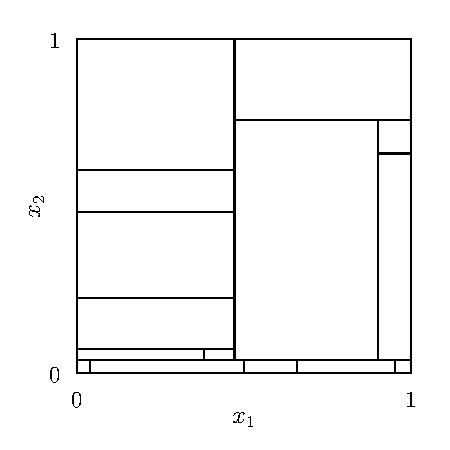
\includegraphics[scale=0.64]{graphics/plot_mondrian_process_1.pdf}
    \caption{$\lambda = 3$}
  \end{subfigure}
  %
  \begin{subfigure}{0.32\textwidth}
    \centering
    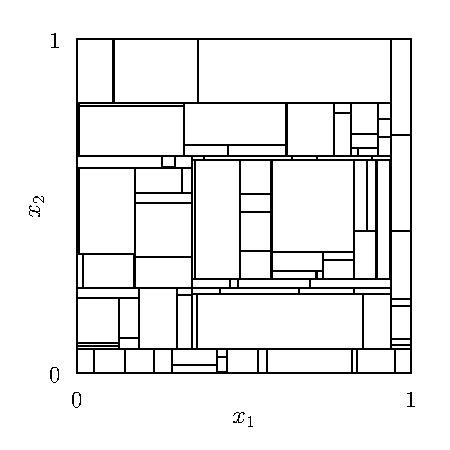
\includegraphics[scale=0.64]{graphics/plot_mondrian_process_2.pdf}
    \caption{$\lambda = 10$}
  \end{subfigure}
  %
  \begin{subfigure}{0.32\textwidth}
    \centering
    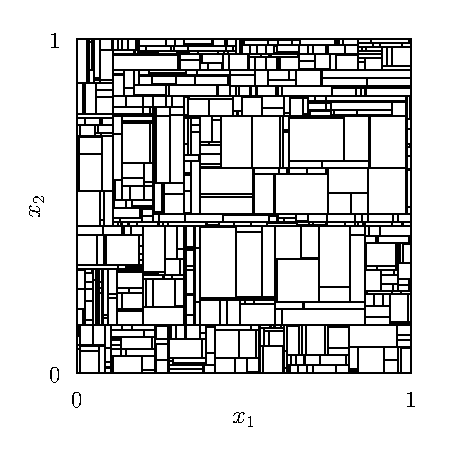
\includegraphics[scale=0.64]{graphics/plot_mondrian_process_3.pdf}
    \caption{$\lambda = 30$}
  \end{subfigure}
  %
  \caption[The Mondrian process]{
    The Mondrian process $T \sim \cM \big( [0,1]^d, \lambda \big)$ with
  $d=2$ and lifetime parameters $\lambda$.}
  \label{fig:mondrian_process}
\end{figure}

\subsection{Data generation}

Throughout this chapter, we assume that the data satisfies
Assumption~\ref{ass:mondrian_data}. We begin with a definition of H{\"o}lder
continuity which will be used for controlling the bias of various estimators.

\begin{definition}[H{\"o}lder continuity]%

  Take $\beta > 0$ and define $\flbeta$ to be the largest integer which is
  strictly less than $\beta$. We say a function $g: [0,1]^d \to \R$ is
  $\beta$-H{\"o}lder continuous and write $g \in \cH^\beta$ if $g$ is $\flbeta$
  times differentiable and
  $\max_{|\nu| = \flbeta}
  \left| \partial^\nu g(x) - \partial^{\nu} g(x') \right|
  \leq C \|x-x'\|_2^{\beta - \flbeta}$
  for some constant $C > 0$ and all $x, x' \in [0,1]^d$. Here, $\nu \in \N^d$
  is a multi-index with $|\nu| = \sum_{j=1}^d \nu_j$ and
  $\partial^{\nu} g(x) = \partial^{|\nu|} g(x) \big/
  \prod_{j=1}^d \partial x_j^{\nu_j}$. We say $g$ is Lipschitz if $g \in \cH^1$.

\end{definition}

\begin{assumption}[Data generation]%
  \label{ass:mondrian_data}

  Fix $d \geq 1$ and let $(X_i, Y_i)$ be i.i.d.\ samples from a distribution on
  $\R^d \times \R$, writing $\bX = (X_1, \ldots, X_n)$ and
  $\bY = (Y_1, \ldots, Y_n)$. Suppose $X_i$ has a Lebesgue density function
  $f(x)$ on $[0,1]^d$ which is bounded away from zero and satisfies
  $f \in \cH^\beta$ for some $\beta \geq 1$. Suppose $\E[Y_i^2 \mid X_i]$ is
  bounded, let $\mu(X_i) = \E[Y_i \mid X_i]$, and assume $\mu \in \cH^\beta$.
  Write $\varepsilon_i = Y_i - \mu(X_i)$ and assume
  $\sigma^2(X_i) = \E[\varepsilon_i^2 \mid X_i]$
  is Lipschitz and bounded away from zero.

\end{assumption}

Some comments are in order surrounding Assumption~\ref{ass:mondrian_data}. The
requirement that the covariate density $f(x)$ be strictly positive on all of
$[0,1]^d$ may seem strong, particularly when $d$ is moderately large. However,
since our theory is presented pointwise in $x$, it is sufficient for this to
hold only on some neighborhood of $x$. To see this, note that continuity
implies the density is positive on some hypercube containing $x$. Upon
rescaling the covariates, we can map this hypercube onto $[0,1]^d$. The same
argument of course holds for the H{\"o}lder smoothness assumptions and the
upper and lower bounds on the conditional variance function.

\subsection{Mondrian random forests}
\label{sec:mondrian_forests}

We define the basic Mondrian random forest estimator
\eqref{eq:mondrian_estimator} as in \citet{lakshminarayanan2014mondrian} and
\citet{mourtada2020minimax}, and will later extend it to a debiased version in
Section~\ref{sec:mondrian_debiased}. For a lifetime parameter $\lambda > 0$ and forest
size $B \geq 1$, let $\bT = (T_1, \ldots, T_B)$ be a Mondrian forest where
$T_b \sim \cM\big([0,1]^d, \lambda\big)$ are i.i.d.\ Mondrian trees
which are independent of the data. For $x \in [0,1]^d$, write
$N_b(x) = \sum_{i=1}^{n} \I \left\{ X_i \in T_b(x) \right\}$ for the number of
samples in $T_b(x)$, with $\I$ denoting an indicator function. Then the
Mondrian random forest estimator of $\mu(x)$ is
%
\begin{align}
  \label{eq:mondrian_estimator}
  \hat\mu(x) = \frac{1}{B} \sum_{b=1}^B
  \frac{\sum_{i=1}^n Y_i \, \I\big\{ X_i \in T_b(x) \big\}} {N_b(x)}.
\end{align}
%
If there are no samples $X_i$ in $T_b(x)$ then $N_b(x) = 0$, so we define
$0/0 = 0$ (see Section~\ref{sec:mondrian_app_proofs} for details). To ensure the
bias and variance of the Mondrian random forest estimator converge to zero (see
Section~\ref{sec:mondrian_inference}), and to avoid boundary issues, we impose
some basic conditions on $x$, $\lambda$, and $B$ in
Assumption~\ref{ass:mondrian_estimator}.

\begin{assumption}[Mondrian random forest estimator]%
  \label{ass:mondrian_estimator}
  %
  Suppose $x \in (0,1)^d$ is an interior point of the support of $X_i$,
  $\frac{\lambda^d}{n} \to 0$,
  $\log \lambda \asymp \log n$,
  and $B \asymp n^{\xi}$ for some $\xi \in (0, 1)$,
  which may depend on the dimension $d$ and smoothness $\beta$.
  %
\end{assumption}

Assumption~\ref{ass:mondrian_estimator} implies that the size of the forest $B$ grows
with $n$. For the purpose of mitigating the computational burden, we suggest
the sub-linear polynomial growth $B \asymp n^{\xi}$, satisfying the conditions
imposed in our main results. Large forests usually do not present computational
challenges in practice as the ensemble estimator is easily parallelizable over
the trees. We emphasize places where this ``large forest'' condition is
important to our theory as they arise throughout the chapter.

\section{Inference with Mondrian random forests}%
\label{sec:mondrian_inference}

We begins with a bias--variance decomposition for the Mondrian random
forest estimator:
%
\begin{align}
  \nonumber
  \hat\mu(x) - \mu(x)
  &=
  \Big( \hat\mu(x) - \E \big[ \hat \mu(x) \mid \bX, \bT \big]\Big)
  + \Big( \E \big[ \hat \mu(x) \mid \bX, \bT \big] - \mu(x)\Big) \\
  &=
  \nonumber
  \left(
    \frac{1}{B} \sum_{b=1}^B
    \frac{\sum_{i=1}^n \varepsilon_i \, \I\big\{ X_i \in T_b(x) \big\}} {N_b(x)}
  \right) \\
  \label{eq:mondrian_bias_variance}
  &\quad+
  \left(
    \frac{1}{B} \sum_{b=1}^B
    \frac{\sum_{i=1}^n \big(\mu(X_i) - \mu(x)\big) \,
    \I\big\{ X_i \in T_b(x) \big\}} {N_b(x)}
  \right).
\end{align}
%
Our approach to inference is summarized as follows. Firstly, we provide a
central limit theorem (weak convergence to a Gaussian) for the first
``variance'' term in \eqref{eq:mondrian_bias_variance}. Secondly, we precisely compute
the probability limit of the second ``bias'' term. By ensuring that the
standard deviation dominates the bias, we can conclude that a corresponding
central limit theorem holds for the Mondrian random forest. With an appropriate
estimator for the limiting variance, we establish procedures for valid and
feasible statistical inference on the unknown regression function $\mu(x)$.

We begin with the aforementioned central limit theorem, which forms the core of
our methodology for performing statistical inference. Before stating our main
result, we highlight some of the challenges involved. At first glance, the
summands in the first term in \eqref{eq:mondrian_bias_variance} seem to be independent
over $1 \leq i \leq n$, conditional on the forest $\bT$, depending only on
$X_i$ and $\varepsilon_i$. However, the $N_b(x)$ appearing in the denominator
depends on all $X_i$ simultaneously, violating this independence assumption and
rendering classical central limit theorems inapplicable. A natural preliminary
attempt to resolve this issue is to observe that
%
\begin{align*}
  N_b(x)&=
  \sum_{i=1}^{n} \I\big\{X_i \in T_b(x)\big\}
  \approx n \, \P \big( X_i \in T_b(x) \mid T_b \big)
  \approx n f(x) |T_b(x)|
\end{align*}
%
with high probability. One could attempt to use this by approximating the
estimator with an average of i.i.d.\ random variables, or by employing a
central limit theorem conditional on $\bX$ and $\bT$. However, such an approach
fails because $\E \left[ \frac{1}{|T_b(x)|^2} \right] = \infty$; the possible
existence of small cells causes the law of the inverse cell volume to have
heavy tails. For similar reasons, attempts to directly establish a central
limit theorem based on $2 + \delta$ moments, such as the Lyapunov central limit
theorem, are ineffective.

We circumvent these problems by directly analyzing
$\frac{\I\{N_b(x) \geq 1\}}{N_b(x)}$. We establish concentration properties for
this non-linear function of $X_i$ via the Efron--Stein inequality
\citep[Section 3.1]{boucheron2013concentration} along with a sequence of
somewhat delicate preliminary lemmas regarding inverse moments of truncated
(conditional) binomial random variables. In particular, we show that
$\E \left[ \frac{\I \{N_b(x) \geq 1\}}{N_b(x)} \right]
\lesssim \frac{\lambda^d}{n}$ and
$\E \left[ \frac{\I \{N_b(x) \geq 1\}}{N_b(x)^2} \right]
\lesssim \frac{\lambda^{2d} \log n}{n^2}$.
Asymptotic normality is then established using a central limit theorem for
martingale difference sequences \citep[Theorem~3.2]{hall1980martingale} with
respect to an appropriate filtration. Section~\ref{sec:mondrian_overview_proofs} gives
an overview our proof strategy in which  we further discuss the underlying
challenges, while Section~\ref{sec:mondrian_app_proofs} gives all the technical
details.

\subsection{Central limit theorem}
\label{sec:mondrian_clt}

Theorem~\ref{thm:mondrian_clt} gives our first main result; a central
limit theorem.

\begin{theorem}[Central limit theorem for the centered
  Mondrian random forest estimator]%
  \label{thm:mondrian_clt}
  %
  Suppose Assumptions~\ref{ass:mondrian_data} and \ref{ass:mondrian_estimator} hold,
  $\E[Y_i^4 \mid X_i ]$ is bounded almost surely,
  and $\frac{\lambda^d \log n}{n} \to 0$. Then
  %
  \begin{align*}
    \sqrt{\frac{n}{\lambda^d}}
    \Big( \hat \mu(x) - \E \big[ \hat \mu(x) \mid \bX, \bT \big] \Big)
    &\rightsquigarrow \cN\big(0, \Sigma(x)\big)
    & &\text{where}
    &\Sigma(x) &=
    \frac{\sigma^2(x)}{f(x)} \left( \frac{4 - 4 \log 2}{3 } \right)^d.
  \end{align*}
\end{theorem}

The condition of $B \to \infty$ is crucial, ensuring sufficient ``mixing'' of
different Mondrian cells to escape the heavy-tailed phenomenon detailed in the
preceding discussion. For concreteness, the large forest condition allows us to
deal with expressions such as
$\E \left[ \frac{1}{|T_b(x)| |T_{b'}(x)|} \right]
= \E \left[ \frac{1}{|T_b(x)|} \right] \E \left[ \frac{1}{|T_{b'}(x)|} \right]
\approx \lambda^{2d} < \infty$
where $b \neq b'$, by independence of the trees, rather than the ``no
ensembling'' single tree analog
$\E \left[ \frac{1}{|T_b(x)|^2} \right] = \infty$.

We take this opportunity to contrast Mondrian random forests with more
classical kernel-based smoothing methods. The lifetime $\lambda$ plays a
similar role to the inverse bandwidth in determining the effective sample size
$n / \lambda^d$, and thus the associated rate of convergence. However, due to
the Mondrian process construction, some cells are typically ``too small''
(equivalent to an insufficiently large bandwidth) to give an appropriate
effective sample size. Similarly, classical methods based on non-random
partitioning such as spline estimators \citep{huang2003local,cattaneo2020large}
typically impose a quasi-uniformity assumption to ensure all the cells are of
comparable size, a property which does not hold for the Mondrian process (not
even with probability approaching one).

\subsection*{Bias characterization}

We turn to the second term in \eqref{eq:mondrian_bias_variance}, which captures the bias
of the Mondrian random forest estimator conditional on the covariates $\bX$ and
the forest $\bT$. As such it is a random quantity which, as we will
demonstrate, converges in probability. We precisely characterize the limiting
non-random bias, including high-degree polynomials in $\lambda$ which for now
may seem ignorable. Indeed the magnitude of the bias is determined by its
leading term, typically of order $1/\lambda^2$ whenever $\beta \geq 2$, and
this suffices for ensuring a negligible contribution from the bias with an
appropriate choice of lifetime parameter. However, the advantage of specifying
higher-order bias terms is made apparent in Section~\ref{sec:mondrian_debiased} when we
construct a debiased Mondrian random forest estimator. There, we target and
annihilate the higher-order terms in order to furnish superior estimation and
inference properties.

Theorem~\ref{thm:mondrian_bias} gives our main result on
the bias of the Mondrian random forest estimator.

\begin{theorem}[Bias of the Mondrian random forest estimator]%
  \label{thm:mondrian_bias}
  %
  Suppose Assumptions~\ref{ass:mondrian_data} and \ref{ass:mondrian_estimator} hold.
  Then for each $1 \leq r \leq \lfloor \flbeta / 2 \rfloor$ there exists
  $B_r(x) \in \R$, which is a function only of
  the derivatives of $f$ and $\mu$ at $x$ up to order $2r$, with
  %
  \begin{align*}
    \E \left[ \hat \mu(x) \mid \bX, \bT \right]
    &=
    \mu(x)
    + \sum_{r=1}^{\lfloor \flbeta / 2 \rfloor}
    \frac{B_r(x)}{\lambda^{2r}}
    + O_\P \left(
      \frac{1}{\lambda^\beta}
      + \frac{1}{\lambda \sqrt B}
      + \frac{\log n}{\lambda} \sqrt{\frac{\lambda^d}{n}}
    \right).
  \end{align*}
  %
  Whenever $\beta > 2$ the leading bias is the quadratic term
  %
  \begin{align*}
    \frac{B_1(x)}{\lambda^2}
    &=
    \frac{1}{2 \lambda^2}
    \sum_{j=1}^d \frac{\partial^2 \mu(x)}{\partial x_j^2}
    + \frac{1}{2 \lambda^2}
    \frac{1}{f(x)}
    \sum_{j=1}^{d} \frac{\partial \mu(x)}{\partial x_j}
    \frac{\partial f(x)}{\partial x_j}.
  \end{align*}
  %
  If $X_i \sim \Unif\big([0,1]^d\big)$ then $f(x) = 1$,
  and using multi-index notation we have
  %
  \begin{align*}
    \frac{B_r(x)}{\lambda^{2r}}
    &=
    \frac{1}{\lambda^{2r}} \sum_{|\nu|=r} \partial^{2 \nu} \mu(x)
    \prod_{j=1}^d \frac{1}{\nu_j + 1}.
  \end{align*}
  %
\end{theorem}

In Theorem~\ref{thm:mondrian_bias} we give some explicit examples of
calculating the
limiting bias if $\beta > 2$ or when $X_i$ are uniformly distributed. The
general form of $B_r(x)$ is provided in Section~\ref{sec:mondrian_app_proofs} but
is somewhat unwieldy except in specific situations. Nonetheless the most
important properties are that $B_r(x)$ are non-random and do not depend on the
lifetime $\lambda$, crucial facts for our debiasing procedure given in
Section~\ref{sec:mondrian_debiased}. If the forest size $B$ does not diverge to infinity
then we suffer the first-order bias term $\frac{1}{\lambda \sqrt B}$. This
phenomenon was explained by \citet{mourtada2020minimax}, who noted that it
allows single Mondrian trees to achieve minimax optimality only when
$\beta \in (0, 1]$. In contrast, large forests remove this first-order bias
and as such are optimal for all $\beta \in (0, 2]$.

Using Theorem~\ref{thm:mondrian_clt} and Theorem~\ref{thm:mondrian_bias} together,
along with an appropriate choice of lifetime parameter $\lambda$,
gives a central limit theorem for the Mondrian random forest estimator
which can be used, for example, to build confidence intervals
for the unknown regression function $\mu(x)$
whenever the bias shrinks faster than the standard deviation.
In general this will require
$\frac{1}{\lambda^2} + \frac{1}{\lambda^\beta} + \frac{1}{\lambda \sqrt B}
\ll \sqrt{\frac{\lambda^d}{n}}$,
which can be satisfied by imposing the restrictions
$\lambda \gg n^{\frac{1}{d + 2(2 \wedge \beta)}}$
and $B \gg n^{\frac{2(2 \wedge \beta) - 2}{d + 2(2 \wedge \beta)}}$
on the lifetime $\lambda$ and forest size $B$.
If instead we aim for optimal point estimation,
then balancing the bias and standard deviation requires
$\frac{1}{\lambda^2} + \frac{1}{\lambda^\beta} + \frac{1}{\lambda \sqrt B}
\asymp \sqrt{\frac{\lambda^d}{n}}$,
which can be satisfied by
$\lambda \asymp n^{\frac{1}{d + 2(2 \wedge \beta)}}$
and $B \gtrsim n^{\frac{2(2 \wedge \beta) - 2}{d + 2(2 \wedge \beta)}}$.
Such a choice of $\lambda$ gives the convergence rate
$n^{\frac{-(2 \wedge \beta)}{d + 2(2 \wedge \beta)}}$
which is the minimax-optimal rate of convergence \citep{stone1982optimal}
for $\beta$-H{\"o}lder functions with $\beta \in (0,2]$
as shown by \citet[Theorem~2]{mourtada2020minimax}.
In Section~\ref{sec:mondrian_debiased} we will show how the Mondrian random forest
estimator can be debiased, giving both weaker lifetime conditions for inference
and also improved rates of convergence, under additional smoothness assumptions.

\subsection*{Variance estimation}

The limiting variance $\Sigma(x)$ from the resulting central limit theorem
depends on the unknown quantities $\sigma^2(x)$ and $f(x)$.
To conduct feasible inference, we must therefore first estimate
$\Sigma(x)$. To this end, define
%
\begin{align}
  \label{eq:mondrian_sigma2_hat}
  \hat\sigma^2(x)
  &=
  \frac{1}{B} \sum_{b=1}^{B} \sum_{i=1}^n
  \frac{\big(Y_i - \hat \mu(x)\big)^2 \, \I\{X_i \in T_b(x)\}} {N_b(x)}, \\
  \nonumber
  \hat\Sigma(x)
  &=
  \hat\sigma^2(x) \frac{n}{\lambda^d} \sum_{i=1}^n
  \left( \frac{1}{B} \sum_{b=1}^B \frac{\I\{X_i \in T_b(x)\}}{N_b(x)} \right)^2.
\end{align}
%
In Theorem~\ref{thm:mondrian_variance_estimation} we show that this
estimator is consistent, and establish its rate of convergence.
%
\begin{theorem}[Variance estimation]%
  \label{thm:mondrian_variance_estimation}
  Grant Assumptions~\ref{ass:mondrian_data} and \ref{ass:mondrian_estimator}, and
  suppose $\E[Y_i^4 \mid X_i ]$ is bounded almost surely. Then
  %
  \begin{align*}
    \hat\Sigma(x)
    = \Sigma(x)
    + O_\P \left(
      \frac{(\log n)^{d+1}}{\lambda}
      + \frac{1}{\sqrt B} + \sqrt{\frac{\lambda^d \log n}{n}}
    \right).
  \end{align*}

\end{theorem}

\subsection{Confidence intervals}

Theorem~\ref{thm:mondrian_confidence} shows how to construct valid confidence intervals
for the regression function $\mu(x)$ under the lifetime and forest size
assumptions previously discussed. For details on feasible and practical
selection of the lifetime parameter $\lambda$, see
Section~\ref{sec:mondrian_parameter_selection}.
%
\begin{theorem}[Feasible confidence intervals using a Mondrian random forest]%
  \label{thm:mondrian_confidence}
  %
  Suppose Assumptions~\ref{ass:mondrian_data} and \ref{ass:mondrian_estimator} hold,
  $\E[Y_i^4 \mid X_i ]$ is bounded almost surely,
  and $\frac{\lambda^d \log n}{n} \to 0$. Assume that
  $\lambda \gg n^{\frac{1}{d + 2(2 \wedge \beta)}}$
  and $B \gg n^{\frac{2 (2 \wedge \beta) - 2}{d + 2 (2 \wedge \beta)}}$.
  For a confidence level $\alpha \in (0, 1)$,
  let $q_{1 - \alpha / 2}$ be the normal quantile satisfying
  $\P \left( \cN(0, 1) \leq q_{1 - \alpha / 2} \right) = 1 - \alpha / 2$. Then
  %
  \begin{align*}
    \P \left(
      \mu(x) \in
      \left[
        \hat \mu(x)
        - \sqrt{\frac{\lambda^d}{n}} \hat \Sigma(x)^{1/2}
        q_{1 - \alpha / 2}, \
        \hat \mu(x)
        + \sqrt{\frac{\lambda^d}{n}} \hat \Sigma(x)^{1/2}
        q_{1 - \alpha / 2}
      \right]
    \right)
    \to
    1 - \alpha.
  \end{align*}

\end{theorem}

When coupled with an appropriate lifetime selection method,
Theorem~\ref{thm:mondrian_confidence} gives a fully feasible procedure for uncertainty
quantification in Mondrian random forests. Our procedure requires no adjustment
of the original Mondrian random forest estimator beyond ensuring that the bias
is negligible, and in particular does not rely on sample splitting. The
construction of confidence intervals is just one corollary of the weak
convergence result given in Theorem~\ref{thm:mondrian_clt}, and follows immediately from
Slutsky's theorem with a consistent variance estimator. Other applications
include hypothesis testing on the value of $\mu(x)$ at a design point $x$ by
inversion of the confidence interval, as well as parametric specification
testing by comparison with a $\sqrt{n}$-consistent parametric regression
estimator. The construction of simultaneous confidence intervals for finitely
many points $x_1, \ldots, x_D$ can be accomplished either using standard
multiple testing corrections or by first establishing a multivariate central
limit theorem using the Cram{\'e}r--Wold device
\citep[Chapter~8]{pollard2002user}
and formulating a consistent multivariate variance estimator.

\section{Overview of proof strategy}%
\label{sec:mondrian_overview_proofs}

This section provides some insight into the general approach we use to
establish the main results in the preceding sections. We focus on the technical
innovations forming the core of our arguments, and refer the reader to
Section~\ref{sec:mondrian_app_proofs} for detailed proofs, including those for the
debiased estimator discussed in the upcoming Section~\ref{sec:mondrian_debiased}.

\subsection*{Preliminary results}

The starting point for our proofs is a result characterizing the exact
distribution of the shape of a Mondrian cell $T(x)$. This property is a direct
consequence of the fact that the restriction of a Mondrian process to a subcell
remains a Mondrian process \citep[Fact~2]{mourtada2020minimax}. We have that
%
\begin{align*}
  |T(x)_j|
  &= \left( \frac{E_{j1}}{\lambda} \wedge x_j \right)
  + \left( \frac{E_{j2}}{\lambda} \wedge (1-x_j) \right)
\end{align*}
%
for all $1 \leq j \leq d$, recalling that $T(x)_j$ is the side of the cell
$T(x)$ aligned with axis $j$, and where $E_{j1}$ and $E_{j2}$ are mutually
independent $\Exp(1)$ random variables. Our assumptions that $x \in (0,1)$ and
$\lambda \to \infty$ mean that the boundary terms $x_j$ and $1-x_j$ are
eventually ignorable and so
%
\begin{align*}
  |T(x)_j| &= \frac{E_{j1} + E_{j2}}{\lambda}
\end{align*}
%
with high probability. Controlling the size of the largest cell in the forest
containing $x$ is now straightforward with a union bound, exploiting the sharp
tail decay of the exponential distribution, and thus
%
\begin{align*}
  \max_{1 \leq b \leq B} \max_{1 \leq j \leq d} |T_b(x)_j|
  \lesssim_\P \frac{\log B}{\lambda}.
\end{align*}
%
This shows that up to logarithmic terms, none of the cells in the forest at $x$
are significantly larger than average, ensuring that the Mondrian random forest
estimator is localized around $x$ on the scale of $1/\lambda$, an important
property for the upcoming bias characterization.

Having provided upper bounds for the sizes of Mondrian cells, we also must
establish some lower bounds in order to quantify the ``small cells'' phenomenon
mentioned previously. The first step towards this is to bound the first two
moments of the truncated inverse Mondrian cell volume; we show that
%
\begin{align*}
  \E\left[ 1 \wedge \frac{1}{n |T(x)|} \right]
  &\asymp \frac{\lambda^d}{n}
  &&\text{and}
  &\frac{\lambda^{2d}}{n^2}
  &\lesssim
  \E\left[ 1 \wedge \frac{1}{n^2 |T(x)|^2} \right]
  \lesssim \frac{\lambda^{2d} \log n}{n^2}.
\end{align*}
%
These bounds are computed directly using the exact distribution of $|T(x)|$.
Note that $\E\left[ \frac{1}{|T(x)|^2} \right] = \infty$ because
$\frac{1}{E_{j1} + E_{j2}}$ has only $2 - \delta$ finite moments, so the
truncation is crucial here. Since we nearly have two moments, this
truncation is at the expense of only a logarithmic term. Nonetheless, third and
higher truncated moments will not enjoy such tight bounds, demonstrating both
the fragility of this result and the inadequacy of tools such as the Lyapunov
central limit theorem which require $2 + \delta$ moments.

To conclude this investigation into the small cell phenomenon, we apply the
previous bounds to ensure that the empirical effective sample sizes
$N_b(x) = \sum_{i=1}^{n} \I \left\{ X_i \in T_b(x) \right\}$ are approximately
of the order $n / \lambda^d$ in an appropriate sense; we demonstrate that
%
\begin{align*}
  \E\left[ \frac{\I\{N_b(x) \geq 1\}}{N_b(x)} \right]
  &\lesssim \frac{\lambda^d}{n}
  &&\text{and}
  &\E\left[ \frac{\I\{N_b(x) \geq 1\}}{N_b(x)^2} \right]
  &\lesssim \frac{\lambda^{2d} \log n}{n^2},
\end{align*}
%
as well as similar bounds for mixed terms such as
%
$\E \left[
  \frac{\I\{N_b(x) \geq 1\}}{N_b(x)}
  \frac{\I\{N_{b'}(x) \geq 1\}}{N_{b'}(x)}
\right]
\lesssim \frac{\lambda^{2d}}{n^2}$
%
when $b \neq b'$, which arise from covariance terms across multiple trees. The
proof of this result is involved and technical, and proceeds by induction. The
idea is to construct a class of subcells by taking all possible intersections
of the cells in $T_b$ and $T_{b'}$ (we show two trees here for clarity; there
may be more) and noting that each $N_b(x)$ is the sum of the number of points
in each such refined cell intersected with $T_b(x)$. We then swap out each
refined cell one at a time and replace the number of data points it contains
with its volume multiplied by $n f(x)$, showing that the expectation on the
left hand side does not increase too much using a moment bound for inverse
binomial random variables based on Bernstein's inequality. By induction and
independence of the trees, eventually the problem is reduced to computing
moments of truncated inverse Mondrian cell volumes, as above.

\subsection*{Central limit theorem}

To prove our main central limit theorem result (Theorem~\ref{thm:mondrian_clt}), we use
the martingale central limit theorem given by
\citet[Theorem~3.2]{hall1980martingale}. For each $1 \leq i \leq n$ define
$\cH_{n i}$ to be the filtration generated by $\bT$, $\bX$, and
$(\varepsilon_j : 1 \leq j \leq i)$, noting that
$\cH_{n i} \subseteq \cH_{(n+1)i}$ because $B$ increases as $n$ increases.
Define the $\cH_{n i}$-measurable and square integrable variables
%
\begin{align*}
  S_i(x) &=
  \sqrt{\frac{n}{\lambda^d}} \frac{1}{B} \sum_{b=1}^B
  \frac{\I \{X_i \in T_b(x)\} \varepsilon_i} {N_{b}(x)},
\end{align*}
%
which satisfy the martingale difference property
$\E [ S_i(x) \mid \cH_{n i} ] = 0$. Further,
%
\begin{align*}
  \sqrt{\frac{n}{\lambda^d}}
  \big(
    \hat\mu(x)
    - \E\left[
      \hat\mu(x) \mid \bX, \bT
    \right]
  \big)
  = \sum_{i=1}^n S_i(x).
\end{align*}
%
To establish weak convergence to $\cN\big(0, \Sigma(x)\big)$,
it suffices to check that $\max_i |S_i(x)| \to 0$ in probability,
$\E\left[\max_i S_i(x)^2\right] \lesssim 1$,
and $\sum_i S_i(x)^2 \to \Sigma(x)$ in probability.
Checking the first two of these is straightforward given the denominator moment
bounds derived above. For the third condition, we demonstrate that
$\sum_i S_i(x)^2$ concentrates by checking its variance is vanishing. To do
this, first observe that $S_i(x)^2$ is the square of a sum over the $B$ trees.
Expanding this square, we see that the diagonal terms (where $b = b'$) provide
a negligible contribution due to the large forest assumption. For the other
terms, we apply the law of total variance and the moment bounds detailed
earlier. Here, it is crucial that $b \neq b'$ in order to exploit the
independence of the trees and avoid having to control any higher-moments. The
law of total variance requires that we bound
%
\begin{align*}
  \Var \left[
    \E \left[
      \sum_{i=1}^n \sum_{b=1}^B \sum_{b' \neq b}
      \frac{\I\{X_i \in T_b(x) \cap T_{b'}(x)\} \varepsilon_i^2}
      {N_{b}(x) N_{b'}(x)} \Bigm| \bX, \bY
    \right]
  \right],
\end{align*}
%
which is the variance of a non-linear function of the i.i.d.\ variables
$(X_i, \varepsilon_i)$, and so we apply the Efron--Stein inequality.
The important insight here is that replacing a sample
$(X_i, \varepsilon_i)$ with an independent copy
$(\tilde X_i, \tilde \varepsilon_i)$ can change the value of
$N_b(x)$ by at most one. Further, this can happen only on the event
$\{ X_i \in T_{b}(x) \} \cup \{ \tilde X_i \in T_{b}(x) \}$,
which occurs with probability on the order $1/\lambda^d$
(the expected cell volume).

The final part of the central limit theorem proof is to calculate the limiting
variance $\Sigma(x)$. The penultimate step showed that we must have
%
\begin{align*}
  \Sigma(x)
  &= \lim_{n \to \infty} \sum_{i=1}^n \E \left[S_i(x)^2 \right]
  = \lim_{n \to \infty}
  \frac{n^2}{\lambda^d} \,
  \E \left[
    \frac{\I\{X_i \in T_b(x) \cap T_{b'}(x)\} \varepsilon_i^2}
    {N_{b}(x) N_{b'}(x)}
  \right],
\end{align*}
%
assuming the limit exists, so it remains to check this and calculate the limit.
It is a straightforward but tedious exercise to verify that each term can be
replaced with its conditional expectation given $T_b$ and $T_{b'}$, using some
further properties of the binomial and exponential distributions. This yields
%
\begin{align*}
  \Sigma(x)
  &=
  \frac{\sigma^2(x)}{f(x)}
  \lim_{\lambda \to \infty}
  \frac{1}{\lambda^d}
  \E \left[
    \frac{|T_{b}(x) \cap T_{b'}(x)|}
    {|T_{b}(x)| \, |T_{b'}(x)|}
  \right]
  = \frac{\sigma^2(x)}{f(x)}
  \E \left[
    \frac{(E_{1} \wedge E'_{1}) + (E_{2} \wedge E'_{2})}
    {(E_{1} + E_{2}) (E'_{1} + E'_{2})}
  \right]^d
\end{align*}
%
where $E_1$, $E_2$, $E'_1$, and $E'_2$ are independent $\Exp(1)$,
by the cell shape distribution and independence of the trees. This final
expectation is calculated by integration, using various incomplete gamma
function identities.

\subsection*{Bias characterization}

Our second substantial technical result is the bias characterization
given as Theorem~\ref{thm:mondrian_bias}, in which we precisely
characterize the probability limit of the conditional bias
%
\begin{align*}
  \E \left[ \hat \mu(x) \mid \bX, \bT \right]
  - \mu(x)
  &=
  \frac{1}{B} \sum_{b=1}^B
  \sum_{i=1}^n \big( \mu(X_i) - \mu(x) \big)
  \frac{\I\{X_i \in T_b(x)\}}{N_b(x)}.
\end{align*}
%
The first step in this proof is to pass to the ``infinite forest''
limit by taking an expectation conditional on $\bX$, or equivalently
marginalizing over $\bT$, applying the conditional Markov inequality
to see
%
\begin{align*}
  \big|
  \E \left[ \hat \mu(x) \mid \bX, \bT \right]
  - \E \left[ \hat \mu(x) \mid \bX \right]
  \big|
  &\lesssim_\P
  \frac{1}{\lambda \sqrt B}.
\end{align*}
%
While this may seem a crude approximation, it is already known that fixed-size
Mondrian forests have suboptimal bias properties when compared to forests with
a diverging number of trees. In fact, the error $\frac{1}{\lambda \sqrt B}$
exactly accounts for the first-order bias of individual Mondrian trees noted by
\citet{mourtada2020minimax}.

Next we show that $\E \left[ \hat \mu(x) \mid \bX \right]$ converges in
probability to its expectation, again using the Efron--Stein theorem for this
non-linear function of the i.i.d.\ variables $X_i$. The Lipschitz property of
$\mu$ and the upper bound on the maximum cell size give
$|\mu(X_i) - \mu(x)| \lesssim \max_{1 \leq j \leq d} |T_b(x)_j|
\lesssim_\P \frac{\log B}{\lambda}$
whenever $X_i \in T_b(x)$,
so we combine this with moment bounds for the denominator $N_b(x)$ to see
%
\begin{align*}
  \left|
  \E \left[ \hat \mu(x) \mid \bX \right]
  - \E \left[ \hat \mu(x) \right]
  \right|
  \lesssim_\P
  \frac{\log n}{\lambda} \sqrt{\frac{\lambda^d}{n}}.
\end{align*}

The next step is to approximate the resulting non-random bias
$\E \left[ \hat \mu(x) \right] - \mu(x)$ as a polynomial in $1/\lambda$.
To this end, we firstly apply a concentration-type result for the binomial
distribution to deduce that
%
\begin{align*}
  \E \left[ \frac{\I\{N_b(x) \geq 1\}}{N_b(x)} \Bigm| \bT \right]
  \approx \frac{1}{n \int_{T_b(x)} f(s) \diff s}
\end{align*}
%
in an appropriate sense, and hence,
by conditioning on $\bT$ and $\bX$ without $X_i$, we write
%
\begin{align}
  \label{eq:mondrian_bias_ratio}
  \E \left[ \hat \mu(x) \right] - \mu(x)
  &\approx
  \E \left[
    \frac{\int_{T_b(x)} (\mu(s) - \mu(x)) f(s) \diff s}
    {\int_{T_b(x)} f(s) \diff s}
  \right].
\end{align}
%
Next we apply the multivariate version of Taylor's theorem to the integrands in
both the numerator and the denominator in \eqref{eq:mondrian_bias_ratio}, and then apply
the Maclaurin series of $\frac{1}{1+x}$ and the multinomial theorem to recover
a single polynomial in $1/\lambda$. The error term is on the order of
$1/\lambda^\beta$ and depends on the smoothness of $\mu$ and $f$, and the
polynomial coefficients are given by various expectations involving exponential
random variables. The final step is to verify using symmetry of Mondrian cells
that all the odd monomial coefficients are zero, and to calculate some explicit
examples of the form of the limiting bias.

\section{Debiased Mondrian random forests}%
\label{sec:mondrian_debiased}

In this section we give our next main contribution, proposing a variant of the
Mondrian random forest estimator which corrects for higher-order bias with an
approach based on generalized jackknifing \citep{schucany1977improvement}. This
estimator retains the basic form of a Mondrian random forest estimator in the
sense that it is a linear combination of Mondrian tree estimators, but in this
section we allow for non-identical linear coefficients, some of which may be
negative, and for differing lifetime parameters across the trees. Since the
basic Mondrian random forest estimator is a special case of this more general
debiased version, we will discuss only the latter throughout the rest of the
chapter.

We use the explicit form of the bias given in Theorem~\ref{thm:mondrian_bias} to
construct a debiased version of the Mondrian forest estimator. Let $J \geq 0$
be the bias correction order. As such, with $J=0$ we retain the original
Mondrian forest estimator, with $J=1$ we remove second-order bias, and with
$J = \lfloor\flbeta / 2 \rfloor$ we remove bias terms up to and including order
$2 \lfloor\flbeta / 2 \rfloor$, giving the maximum possible bias reduction
achievable in the H{\"o}lder class $\cH^\beta$. As such, only bias terms of
order $1/\lambda^\beta$ will remain.

For $0 \leq r \leq J$ let $\hat \mu_r(x)$ be a Mondrian forest estimator
based on the trees $T_{b r} \sim \cM\big([0,1]^d, \lambda_r \big)$
for $1 \leq b \leq B$, where $\lambda_r = a_r \lambda$ for some $a_r > 0$
and $\lambda > 0$. Write $\bT$ to denote the collection of all the trees,
and suppose they are mutually independent. We find values of $a_r$ along with
coefficients $\omega_r$ in order to annihilate the leading $J$ bias terms of
the debiased Mondrian random forest estimator
%
\begin{align}
  \label{eq:mondrian_debiased}
  \hat \mu_\rd(x)
  &= \sum_{r=0}^J \omega_r \hat \mu_r(x)
  = \sum_{r=0}^{J} \omega_r
  \frac{1}{B} \sum_{b=1}^B
  \frac{\sum_{i=1}^n Y_i \, \I\big\{ X_i \in T_{r b}(x) \big\}} {N_{r b}(x)}.
\end{align}
%
This ensemble estimator retains the ``forest'' structure of the original
estimators, but with varying lifetime parameters $\lambda_r$ and coefficients
$\omega_r$. Thus by Theorem~\ref{thm:mondrian_bias} we want to solve
%
\begin{align*}
  \sum_{r=0}^{J} \omega_r
  \left( \mu(x) + \sum_{s=1}^{J} \frac{B_{s}(x)}{a_r^{2s} \lambda^{2s}} \right)
  &= \mu(x)
\end{align*}
%
for all $\lambda$, or equivalently the system of linear equations
$\sum_{r=0}^{J} \omega_r = 1$
and $\sum_{r=0}^{J} \omega_r a_r^{-2s} = 0$ for each $1 \leq s \leq J$.
We solve these as follows. Define the $(J+1) \times (J+1)$ Vandermonde matrix
$A_{r s} = a_{r-1}^{2-2s}$,
and let $\omega = (\omega_0, \ldots, \omega_J)^\T \in \R^{J+1}$
and $e_0 = (1, 0, \ldots, 0)^\T \in \R^{J+1}$.
Then a solution for the debiasing coefficients is given by
$\omega = A^{-1} e_0$ whenever $A$ is non-singular.
In practice we can take $a_r$ to be a fixed geometric or arithmetic sequence
to ensure this is the case, appealing to the Vandermonde determinant formula:
$\det A = \prod_{0 \leq r < s \leq J} (a_r^{-2} - a_s^{-2})
\neq 0$ whenever $a_r$ are distinct. For example, we could set
$a_r = (1 + \gamma)^r$ or $a_r = 1 + \gamma r$ for some $\gamma > 0$.
Because we assume $\beta$, and therefore the choice of $J$, do not
depend on $n$, there is no need to quantify
the invertibility of $A$ by, for example, bounding its eigenvalues
away from zero as a function of $J$.

\subsection{Central limit theorem}

In Theorem~\ref{thm:mondrian_clt_debiased}, we verify that a central
limit theorem holds for the debiased
random forest estimator $\hat\mu_\rd(x)$ and give its limiting variance.
The strategy and challenges associated with proving
Theorem~\ref{thm:mondrian_clt_debiased} are identical to those discussed earlier
surrounding Theorem~\ref{thm:mondrian_clt}. In fact in Section~\ref{sec:mondrian_app_proofs}
we provide a direct proof only for Theorem~\ref{thm:mondrian_clt_debiased}
and deduce Theorem~\ref{thm:mondrian_clt} as a special case.

\begin{theorem}[Central limit theorem for the
  debiased Mondrian random forest estimator]%
  \label{thm:mondrian_clt_debiased}
  %
  Suppose Assumptions~\ref{ass:mondrian_data} and \ref{ass:mondrian_estimator} hold,
  $\E[Y_i^4 \mid X_i ]$ is bounded,
  and $\frac{\lambda^d \log n}{n} \to 0$. Then
  %
  \begin{align*}
    \sqrt{\frac{n}{\lambda^d}}
    \Big(
      \hat \mu_\rd(x)
      - \E \big[ \hat \mu_\rd(x) \mid \bX, \bT \big]
    \Big)
    &\rightsquigarrow
    \cN\big(0, \Sigma_\rd(x)\big)
  \end{align*}
  %
  where, with $\ell_{r r'} = \frac{2 a_r}{3} \left( 1 - \frac{a_{r}}{a_{r'}}
  \log\left(\frac{a_{r'}}{a_{r}} + 1\right) \right)$,
  the limiting variance is
  %
  \begin{align*}
    \Sigma_\rd(x)
    &=
    \frac{\sigma^2(x)}{f(x)}
    \sum_{r=0}^{J} \sum_{r'=0}^{J} \omega_r \omega_{r'}
    \left( \ell_{r r'} + \ell_{r' r} \right)^d.
  \end{align*}
  %
\end{theorem}

It is easy to verify that in the case of no debiasing we have
$J=0$ and $a_0 = \omega_0 = 1$, yielding
$\Sigma_\rd(x) = \Sigma(x)$, and recovering Theorem~\ref{thm:mondrian_clt}.

\subsection*{Bias characterization}

In Theorem~\ref{thm:mondrian_bias_debiased} we verify that this debiasing
procedure does indeed annihilate the desired bias terms, and its proof is a
consequence of Theorem~\ref{thm:mondrian_bias} and the construction of the
debiased Mondrian random forest estimator $\hat\mu_\rd(x)$.

\begin{theorem}[Bias of the debiased Mondrian random forest estimator]%
  \label{thm:mondrian_bias_debiased}
  Suppose Assumptions~\ref{ass:mondrian_data} and \ref{ass:mondrian_estimator} hold.
  Then using the notation of Theorem~\ref{thm:mondrian_bias} and with
  $\bar\omega = \sum_{r=0}^J \omega_r a_r^{-2J - 2}$,
  %
  \begin{align*}
    \E \big[ \hat \mu_\rd(x) \mid \bX, \bT \big]
    &= \mu(x) + \I\{2J+2 < \beta \}
    \frac{\bar\omega B_{J+1}(x)}{\lambda^{2J + 2}} \\
    &\quad+
    O_\P \left(
      \frac{1}{\lambda^{2J + 4}}
      + \frac{1}{\lambda^\beta}
      + \frac{1}{\lambda \sqrt B}
      + \frac{\log n}{\lambda} \sqrt{\frac{\lambda^d}{n}}
    \right).
  \end{align*}
  %
\end{theorem}

Theorem~\ref{thm:mondrian_bias_debiased} has the following consequence:
the leading bias term is characterized in terms of
$B_{J+1}(x)$ whenever $J < \beta/2 - 1$,
or equivalently $J < \lfloor \flbeta/2 \rfloor$,
that is, the debiasing order
$J$ does not exhaust the H{\"o}lder smoothness $\beta$.
If this condition does not hold, then the estimator is
fully debiased, and the resulting leading bias
term is bounded above by $1/\lambda^\beta$ up to constants,
but its form is left unspecified.

\subsection*{Variance estimation}

As before, we propose a variance estimator in order to conduct feasible
inference and show that it is consistent.
With $\hat\sigma^2(x)$ as in \eqref{eq:mondrian_sigma2_hat}
in Section~\ref{sec:mondrian_inference}, define the estimator
%
\begin{align}
  \label{eq:mondrian_debiased_variance_estimator}
  \hat\Sigma_\rd(x)
  &=
  \hat\sigma^2(x)
  \frac{n}{\lambda^d}
  \sum_{i=1}^n
  \left(
    \sum_{r=0}^J
    \omega_r
    \frac{1}{B}
    \sum_{b=1}^B
    \frac{\I\{X_i \in T_{r b}(x)\}}
    {N_{r b}(x)}
  \right)^2.
\end{align}
%
\begin{theorem}[Variance estimation]%
  \label{thm:mondrian_variance_estimation_debiased}
  Grant Assumptions~\ref{ass:mondrian_data} and \ref{ass:mondrian_estimator}, and
  suppose $\E[Y_i^4 \mid X_i ]$ is bounded almost surely. Then
  %
  \begin{align*}
    \hat\Sigma_\rd(x)
    = \Sigma_\rd(x)
    + O_\P \left(
      \frac{(\log n)^{d+1}}{\lambda}
      + \frac{1}{\sqrt B}
      + \sqrt{\frac{\lambda^d \log n}{n}}
    \right).
  \end{align*}
  %
\end{theorem}

\subsection{Confidence intervals}

In analogy to Section~\ref{sec:mondrian_inference},
we now demonstrate the construction of feasible valid confidence
intervals using the debiased Mondrian random forest estimator
in Theorem~\ref{thm:mondrian_confidence_debiased}.
Once again we must ensure that the bias
(now significantly reduced due to our debiasing procedure)
is negligible when compared to the standard deviation
(which is of the same order as before).
We assume for simplicity that the estimator has been fully
debiased by setting $J \geq \lfloor \flbeta / 2\rfloor$
to yield a leading bias of order $1/\lambda^\beta$,
but intermediate ``partially debiased'' versions can easily
be provided, with leading bias terms of order
$1/\lambda^{\beta \wedge (2J+2)}$ in general.
We thus require
$\frac{1}{\lambda^\beta} + \frac{1}{\lambda \sqrt B}
\ll \sqrt{\frac{\lambda^d}{n}}$,
which can be satisfied by imposing the restrictions
$\lambda \gg n^{\frac{1}{d + 2 \beta}}$
and $B \gg n^{\frac{2\beta - 2}{d + 2\beta}}$
on the lifetime parameter $\lambda$
and forest size $B$.

\begin{theorem}[Feasible confidence intervals using a
  debiased Mondrian random forest]%
  \label{thm:mondrian_confidence_debiased}
  %
  Suppose Assumptions~\ref{ass:mondrian_data} and \ref{ass:mondrian_estimator} hold,
  $\E[Y_i^4 \mid X_i ]$ is bounded,
  and $\frac{\lambda^d \log n}{n} \to 0$.
  Fix $J \geq \lfloor \flbeta / 2 \rfloor$ and assume that
  $\lambda \gg n^{\frac{1}{d + 2 \beta}}$
  and $B \gg n^{\frac{2 \beta - 2}{d + 2 \beta}}$.
  For a confidence level $\alpha \in (0, 1)$,
  let $q_{1 - \alpha / 2}$ be as in Theorem~\ref{thm:mondrian_confidence}. Then
  %
  \begin{align*}
    \P \left(
      \mu(x) \in
      \left[
        \hat \mu_\rd(x)
        - \sqrt{\frac{\lambda^d}{n}} \hat \Sigma_\rd(x)^{1/2}
        q_{1 - \alpha / 2}, \
        \hat \mu_\rd(x)
        + \sqrt{\frac{\lambda^d}{n}} \hat \Sigma_\rd(x)^{1/2}
        q_{1 - \alpha / 2}
      \right]
    \right)
    \to
    1 - \alpha.
  \end{align*}

\end{theorem}

One important benefit of our debiasing technique is made clear in
Theorem~\ref{thm:mondrian_confidence_debiased}: the restrictions imposed on the lifetime
parameter $\lambda$ are substantially relaxed, especially in smooth classes
with large $\beta$. As well as the high-level of benefit of relaxed conditions,
this is also useful for practical selection of appropriate lifetimes for
estimation and inference respectively; see
Section~\ref{sec:mondrian_parameter_selection} for more details. Nonetheless, such
improvements do not come without concession. The limiting variance
$\Sigma_\rd(x)$ of the debiased estimator is larger than that of the unbiased
version (the extent of this increase depends on the choice of the debiasing
parameters $a_r$), leading to wider confidence intervals and larger estimation
error in small samples despite the theoretical asymptotic improvements.

\subsection{Minimax optimality}

Our final result Theorem~\ref{thm:mondrian_minimax} shows that,
when using an appropriate sequence of lifetime parameters $\lambda$,
the debiased Mondrian random forest estimator
achieves, up to constants, the minimax-optimal rate of convergence
for estimating a regression function $\mu \in \cH^\beta$
in $d$ dimensions \citep{stone1982optimal}.
This result holds for all $d \geq 1$ and all $\beta > 0$,
complementing a previous result established only for $\beta \in (0, 2]$
by \citet{mourtada2020minimax}.
%
\begin{theorem}[Minimax optimality of the debiased
  Mondrian random forest estimator]%
  \label{thm:mondrian_minimax}
  Grant Assumptions~\ref{ass:mondrian_data} and \ref{ass:mondrian_estimator},
  and let $J \geq \lfloor \flbeta / 2 \rfloor$,
  $\lambda \asymp n^{\frac{1}{d + 2 \beta}}$, and
  $B \gtrsim n^{\frac{2 \beta - 2}{d + 2 \beta}}$. Then
  %
  \begin{align*}
    \E \left[
      \big( \hat \mu_\rd(x) - \mu(x) \big)^2
    \right]^{1/2}
    &\lesssim
    \sqrt{\frac{\lambda^d}{n}}
    + \frac{1}{\lambda^\beta}
    + \frac{1}{\lambda \sqrt B}
    \lesssim
    n^{-\frac{\beta}{d + 2 \beta}}.
  \end{align*}
  %
\end{theorem}

The sequence of lifetime parameters $\lambda$ required in
Theorem~\ref{thm:mondrian_minimax} are chosen to balance the bias and standard
deviation bounds implied by Theorem~\ref{thm:mondrian_bias_debiased} and
Theorem~\ref{thm:mondrian_clt_debiased} respectively, in order to minimize the pointwise
mean squared error. While selecting an optimal debiasing order $J$ needs only
knowledge of an upper bound on the smoothness $\beta$, choosing an optimal
sequence of $\lambda$ values does assume that $\beta$ is known a priori. The
problem of adapting to $\beta$ from data is challenging and beyond the scope of
this chapter; we provide some practical advice for tuning parameter
selection in Section~\ref{sec:mondrian_parameter_selection}.

Theorem~\ref{thm:mondrian_minimax} complements the minimaxity results proven by
\citet{mourtada2020minimax} for Mondrian trees (with $\beta \leq 1$) and for
Mondrian random forests (with $\beta \leq 2$), with one modification: our
version is stated in pointwise rather than integrated mean squared error. This
is because our debiasing procedure is designed to handle interior smoothing
bias and as such does not provide any correction for boundary bias. We leave
the development of such boundary corrections to future work, but constructions
similar to higher-order boundary-correcting kernels should be possible. If the
region of integration is a compact set in the interior of $[0,1]^d$, then we do
obtain an optimal integrated mean squared error bound: if $\delta \in (0, 1/2)$
is fixed then under the same conditions as Theorem~\ref{thm:mondrian_minimax},
%
\begin{align*}
  \E \left[
    \int_{[\delta, 1-\delta]^d}
    \big(
      \hat \mu_\rd(x)
      - \mu(x)
    \big)^2
    \diff x
  \right]^{1/2}
  &\lesssim
  \sqrt{\frac{\lambda^d}{n}}
  + \frac{1}{\lambda^\beta}
  + \frac{1}{\lambda \sqrt B}
  \lesssim
  n^{-\frac{\beta}{d + 2 \beta}}.
\end{align*}

\subsection{Interpretation}

The debiased Mondrian random forest estimator defined in \eqref{eq:mondrian_debiased} is
a linear combination of Mondrian random forests, and as such contains both a
sum over $0 \leq r \leq J$, representing the debiasing procedure, and a sum
over $1 \leq b \leq B$, representing the forest averaging. We have thus far
been interpreting this estimator as a debiased version of the standard Mondrian
random forest given in \eqref{eq:mondrian_estimator}, but it is
equally valid to swap the order of these sums. This gives rise to an
alternative point of view: we replace each Mondrian random tree with a
``debiased'' version, and then take a forest of such modified trees. This
perspective is more in line with existing techniques for constructing
randomized ensembles, where the outermost operation represents a $B$-fold
average of randomized base learners, not necessarily locally constant decision
trees, each of which has a small bias component \citep{caruana2004ensemble,
zhou2019deep, friedberg2020local}.

\section{Tuning parameter selection}%
\label{sec:mondrian_parameter_selection}

We discuss various procedures for selecting the parameters involved in fitting
a debiased Mondrian random forest; namely the base lifetime parameter
$\lambda$, the number of trees in each forest $B$, the bias correction order
$J$, and the debiasing scale parameters $a_r$ for $0 \leq r \leq J$.

\subsection{Selecting the base lifetime parameter
\texorpdfstring{$\lambda$}{lambda}}%
\label{sec:mondrian_lifetime_selection}

The most important parameter is the base Mondrian lifetime parameter $\lambda$,
which plays the role of a complexity parameter and thus governs the overall
bias--variance trade-off of the estimator. Correct tuning of $\lambda$ is
especially important in two main respects:
%
firstly, in order to use the central limit theorem established in
Theorem~\ref{thm:mondrian_clt_debiased}, we must have that the bias converges to zero,
requiring $\lambda \gg n^{\frac{1}{d + 2\beta}}$.
%
Secondly, the minimax optimality result of Theorem~\ref{thm:mondrian_minimax}
is valid only in the regime $\lambda \asymp n^{\frac{1}{d + 2\beta}}$, and thus
requires careful determination in the more realistic finite-sample setting. For
clarity, in this section we use the notation $\hat\mu_\rd(x; \lambda, J)$ for
the debiased Mondrian random forest with lifetime $\lambda$ and debiasing order
$J$ as in \eqref{eq:mondrian_debiased}.
Similarly write $\hat\Sigma_\rd(x; \lambda, J)$ for the associated
variance estimator given in \eqref{eq:mondrian_debiased_variance_estimator}.

For minimax-optimal point estimation when $\beta$ is known,
choose any sequence $\lambda \asymp n^{\frac{1}{d + 2\beta}}$
and use $\hat\mu_\rd(x; \lambda, J)$ with $J = \lfloor \flbeta / 2 \rfloor$,
following the theory given in Theorem~\ref{thm:mondrian_minimax}.
For an explicit example of how to choose the lifetime, one can instead use
$\hat\mu_\rd\big(x; \hat\lambda_{\AIMSE}(J-1), J-1\big)$
so that the leading bias is explicitly characterized by
Theorem~\ref{thm:mondrian_bias_debiased},
and with $\hat\lambda_{\AIMSE}(J-1)$ as defined below.
This is no longer minimax-optimal as $J-1 < J$
does not satisfy the conditions of Theorem~\ref{thm:mondrian_minimax}.

For performing inference, a more careful procedure is required;
we suggest the following method assuming $\beta > 2$.
Set $J = \lfloor \flbeta / 2 \rfloor$ as before,
and use $\hat\mu_\rd\big(x; \hat\lambda_{\AIMSE}(J-1), J\big)$
and $\hat\Sigma_\rd\big(x; \hat\lambda_{\AIMSE}(J-1), J\big)$
to construct a confidence interval.
The reasoning for this is that we select a lifetime tailored for a more biased
estimator than we actually use. This results in an inflated lifetime estimate,
guaranteeing the resulting bias is negligible when it is plugged into the fully
debiased estimator. This approach to tuning parameter selection and debiasing
for valid nonparametric inference corresponds to an application of robust bias
correction \citep{calonico2018effect,calonico2022coverage},
where the point estimator is bias-corrected
and the robust standard error estimator incorporates the additional
sampling variability introduced by the bias correction.
This leads to a more refined distributional approximation
but does not necessarily exhaust the underlying
smoothness of the regression function.
An alternative inference approach based on Lepskii's method
\citep{lepskii1992asymptotically,birge2001alternative}
could be developed with the latter goal in mind.

It remains to propose a concrete method for computing $\hat\lambda_{\AIMSE}(J)$
in the finite-sample setting; we suggest two such procedures based on plug-in
selection with polynomial estimation and cross-validation respectively,
building on classical ideas from the nonparametric
smoothing literature \citep{fan2020statistical}.

\subsubsection*{Lifetime selection with polynomial estimation}

Firstly suppose $X_i \sim \Unif\big([0,1]^d\big)$
and that the leading bias of $\hat\mu_\rd(x)$ is well approximated by an
additively separable function so that,
writing $\partial^{2 J + 2}_j \mu(x)$
for $\partial^{2 J + 2}_j \mu(x) / \partial x_j^{2 J + 2}$,
%
\begin{align*}
  \frac{\bar \omega B_{J+1}(x)}{\lambda^{2 J + 2}}
  &\approx
  \frac{1}{\lambda^{2 J + 2}}
  \frac{\bar \omega }{J + 2}
  \sum_{j=1}^d
  \partial^{2 J + 2}_j \mu(x).
\end{align*}
%
Now suppose the model is homoscedastic so $\sigma^2(x) = \sigma^2$ and
the limiting variance of $\hat\mu_\rd$ is
%
\begin{align*}
  \frac{\lambda^d}{n}
  \Sigma_\rd(x)
  &=
  \frac{\lambda^d \sigma^2}{n}
  \sum_{r=0}^{J}
  \sum_{r'=0}^{J}
  \omega_r
  \omega_{r'}
  \left( \ell_{r r'} + \ell_{r' r} \right)^d.
\end{align*}
%
The asymptotic integrated mean squared error (AIMSE) is
%
\begin{align*}
  \AIMSE(\lambda, J)
  &=
  \frac{1}{\lambda^{4 J + 4}}
  \frac{\bar \omega^2}{(J + 2)^2}
  \int_{[0,1]^d}
  \left(
    \sum_{j=1}^d
    \partial^{2 J + 2}_j \mu(x)
  \right)^2
  \diff x \\
  &\quad+
  \frac{\lambda^d \sigma^2}{n}
  \sum_{r=0}^{J}
  \sum_{r'=0}^{J}
  \omega_r
  \omega_{r'}
  \left( \ell_{r r'} + \ell_{r' r} \right)^d.
\end{align*}
%
Minimizing over $\lambda > 0$ yields the AIMSE-optimal lifetime parameter
%
\begin{align*}
  \lambda_{\AIMSE}(J)
  &=
  \left(
    \frac{
      \frac{(4 J + 4) \bar \omega^2}{(J + 2)^2}
      n \int_{[0,1]^d}
      \left(
        \sum_{j=1}^d
        \partial^{2 J + 2}_j \mu(x)
      \right)^2
      \diff x
    }{
      d \sigma^2
      \sum_{r=0}^{J}
      \sum_{r'=0}^{J}
      \omega_r
      \omega_{r'}
      \left( \ell_{r r'} + \ell_{r' r} \right)^d
    }
  \right)^{\frac{1}{4 J + 4 + d}}.
\end{align*}
%
An estimator of $\lambda_{\AIMSE}(J)$ is therefore given by
%
\begin{align*}
  \hat\lambda_{\AIMSE}(J)
  &=
  \left(
    \frac{
      \frac{(4 J + 4) \bar \omega^2}{(J + 2)^2}
      \sum_{i=1}^n
      \left(
        \sum_{j=1}^d
        \partial^{2 J + 2}_j \hat\mu(X_i)
      \right)^2
    }{
      d \hat\sigma^2
      \sum_{r=0}^{J}
      \sum_{r'=0}^{J}
      \omega_r
      \omega_{r'}
      \left( \ell_{r r'} + \ell_{r' r} \right)^d
    }
  \right)^{\frac{1}{4 J + 4 + d}}
\end{align*}
%
for some preliminary estimators
$\partial^{2 J + 2}_j \hat\mu(x)$ and $\hat\sigma^2$.
These can be obtained by fitting a global polynomial regression
to the data of order $2 J + 4$ without interaction terms.
To do this, define the $n \times ((2 J + 4)d + 1)$ design matrix $P$ with rows
%
\begin{align*}
  P_i = \big(
    1, X_{i1}, X_{i1}^2, \ldots, X_{i1}^{2 J + 4},
    X_{i2}, X_{i2}^2, \ldots, X_{i2}^{2 J + 4},
    \ldots,
    X_{id}, X_{id}^2, \ldots, X_{id}^{2 J + 4}
  \big),
\end{align*}
%
and let
%
$P_x = \big(
  1, x_{1}, x_{1}^2, \ldots, x_{1}^{2 J + 4},
  x_{2}, x_{2}^2, \ldots, x_{2}^{2 J + 4},
  \ldots,
  x_{d}, x_{d}^2, \ldots, x_{d}^{2 J + 4}
\big).
$
%
Then we define the derivative estimator as
%
\begin{align*}
  \partial^{2 J + 2}_j \hat\mu(x)
  &=
  \partial^{2 J + 2}_j P_x
  \big( P^\T P \big)^{-1}
  P^\T \bY \\
  &=
  (2J + 2)!
  \left(
    0_{1 + (j-1)(2 J + 4) + (2J + 1)},
    1, x_j, x_j^2 / 2,
    0_{(d-j)(2 J + 4)}
  \right)
  \big( P^\T P \big)^{-1}
  P^\T \bY,
\end{align*}
%
and the variance estimator $\hat\sigma^2$ is
based on the residual sum of squared errors of this model:
%
\begin{align*}
  \hat\sigma^2
  &=
  \frac{1}{n - (2J + 4)d - 1}
  \big(
    \bY^\T \bY
    - \bY^\T P \big( P^\T P \big)^{-1} P^\T \bY
  \big).
\end{align*}

\subsubsection*{Lifetime selection with cross-validation}

As an alternative to the analytic plug-in methods described above, one can use
a cross-validation approach. While leave-one-out cross-validation (LOOCV) can
be applied directly \citep{fan2020statistical},
the linear smoother structure of the (debiased) Mondrian
random forest estimator allows a computationally simpler formulation. Writing
$\hat\mu_\rd^{-i}(x)$ for a debiased Mondrian random forest estimator fitted
without the $i$th data sample, it is easy to show that
%
\begin{align*}
  \LOOCV(\lambda, J)
  &=
  \frac{1}{n}
  \sum_{i=1}^{n}
  \left( Y_i - \hat\mu_\rd^{-i}(X_i) \right)^2 \\
  &=
  \frac{1}{n}
  \sum_{i=1}^{n}
  \left(
    \sum_{r=0}^{J}
    \omega_r
    \frac{1}{B}
    \sum_{b=1}^{B}
    \frac{1}{1 - 1/N_{r b}(X_i)}
    \left( Y_i -
      \sum_{j=1}^{n}
      \frac{ Y_j \I \left\{ X_j \in T_{r b}(X_i) \right\}}
      {N_{r b}(X_i)}
    \right)
  \right)^{2},
\end{align*}
%
avoiding refitting the model leaving each sample out in turn.
Supposing $X_i \sim \Unif\big([0,1]^d\big)$ and
replacing $1/N_{r b}(X_i)$ with their average expectation
$ \frac{1}{J+1} \sum_{r=0}^{J} \E \left[ 1/N_{r b}(X_i) \right]
\approx \bar a^d \lambda^d / n$
where $\bar a^d = \frac{1}{J+1} \sum_{r=0}^{J} a_r^d$
gives the generalized cross-validation (GCV) formula
%
\begin{align}
  \label{eq:mondrian_gcv}
  \GCV(\lambda, J)
  &=
  \frac{1}{n}
  \sum_{i=1}^{n}
  \left(
    \frac{Y_i - \hat\mu_\rd(X_i)}
    {1 - \bar a^d \lambda^d / n}
  \right)^2.
\end{align}
%
The lifetime can then be selected by computing
either $\hat\lambda_{\LOOCV} \in \argmin_\lambda \LOOCV(\lambda, J)$
or $\hat\lambda_{\GCV} \in \argmin_\lambda \GCV(\lambda, J)$.
See Section~\ref{sec:mondrian_weather} for a practical illustration.

\subsection{Choosing the number \texorpdfstring{$B$}{B} of trees
in each forest}%

The next parameter to choose is the number of trees in each forest, $B$.
If no debiasing is applied, we suggest taking
$B = \sqrt{n}$ to satisfy the constraint in Theorem~\ref{thm:mondrian_confidence}.
If debiasing is used then we recommend setting
$B = n^{\frac{2J-1}{2J}}$, consistent with Theorem~\ref{thm:mondrian_confidence_debiased}
and Theorem~\ref{thm:mondrian_minimax}.

\subsection{Setting the debiasing order \texorpdfstring{$J$}{J}}%

When constructing a debiased Mondrian random forest estimator, one must decide
how many orders of bias to remove. This requires some form of
oracle knowledge of the H{\"o}lder smoothness of $\mu$ and $f$, which is in
practice very difficult to estimate statistically. As such we recommend
removing only the first one or two bias terms, taking $J \in \{0,1,2\}$ to
avoid overly inflating the variance of the estimator.

\subsection{Selecting the debiasing coefficients}%

As in Section~\ref{sec:mondrian_debiased}, we take $a_r$ to be a fixed
geometric or arithmetic sequence. For example, one could set
$a_r = (1+\gamma)^r$ or $a_r = 1 + \gamma r$ for some $\gamma > 0$.
We suggest taking $a_r = 1.05^r$.

\section{Illustrative example: weather forecasting}%
\label{sec:mondrian_weather}

To demonstrate our methodology for estimation and inference with Mondrian random
forests, we consider a simple application
to a weather forecasting problem. We emphasize that the main aim of this
section is to provide intuition and understanding for how a Mondrian random
forest may be used in practice, and we refrain from an in-depth analysis of the
specific results obtained. Indeed, our core assumption of i.i.d.\ data is almost
certainly
violated when treating weather data, due to the inherent time-series structure
of the sequential observations.
Nonetheless, we use data from the \cite{bureau2017daily}, containing daily
weather
information from the years 2007--2017, at 49 different
locations across Australia, with a total of $n = 125\,927$ samples.

\begin{figure}[t]
  \centering
  \begin{subfigure}{0.49\textwidth}
    \centering
    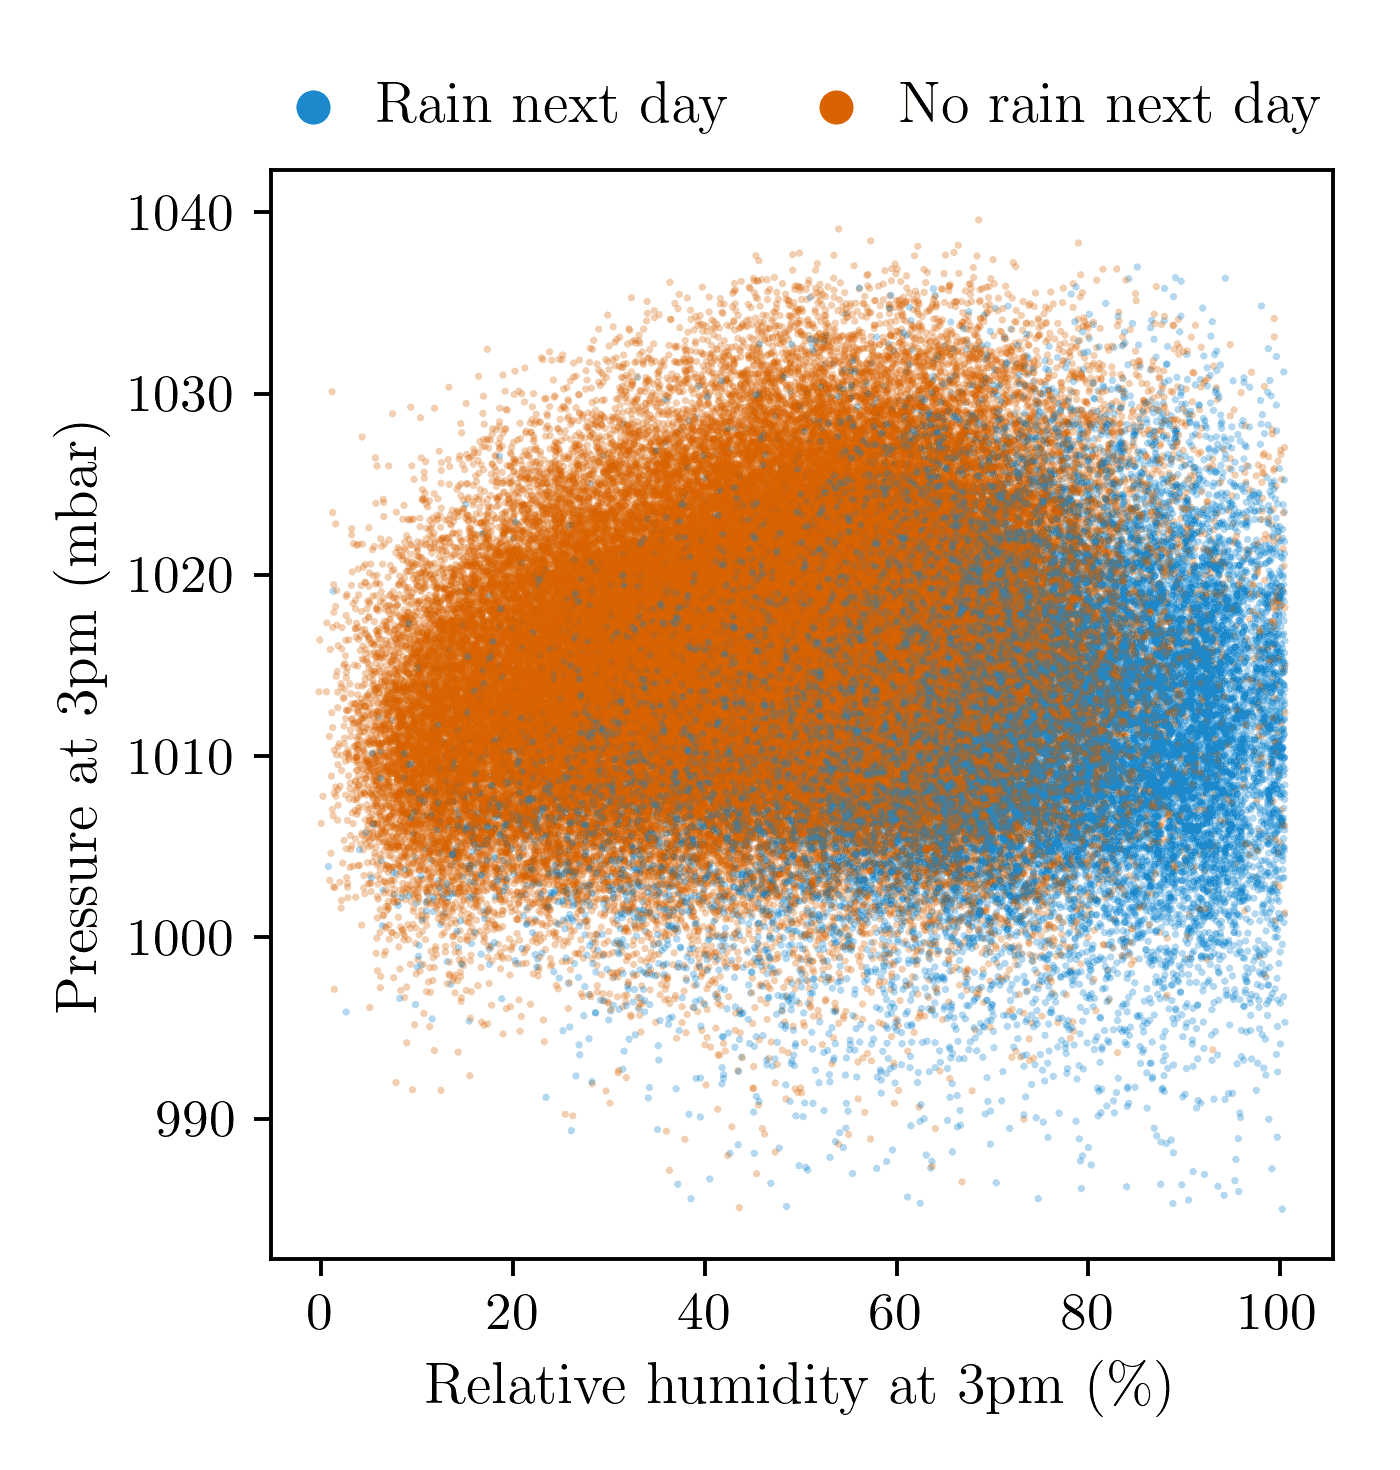
\includegraphics[scale=0.64]{graphics/weather_data.png}%
  \end{subfigure}
  \begin{subfigure}{0.49\textwidth}
    \centering
    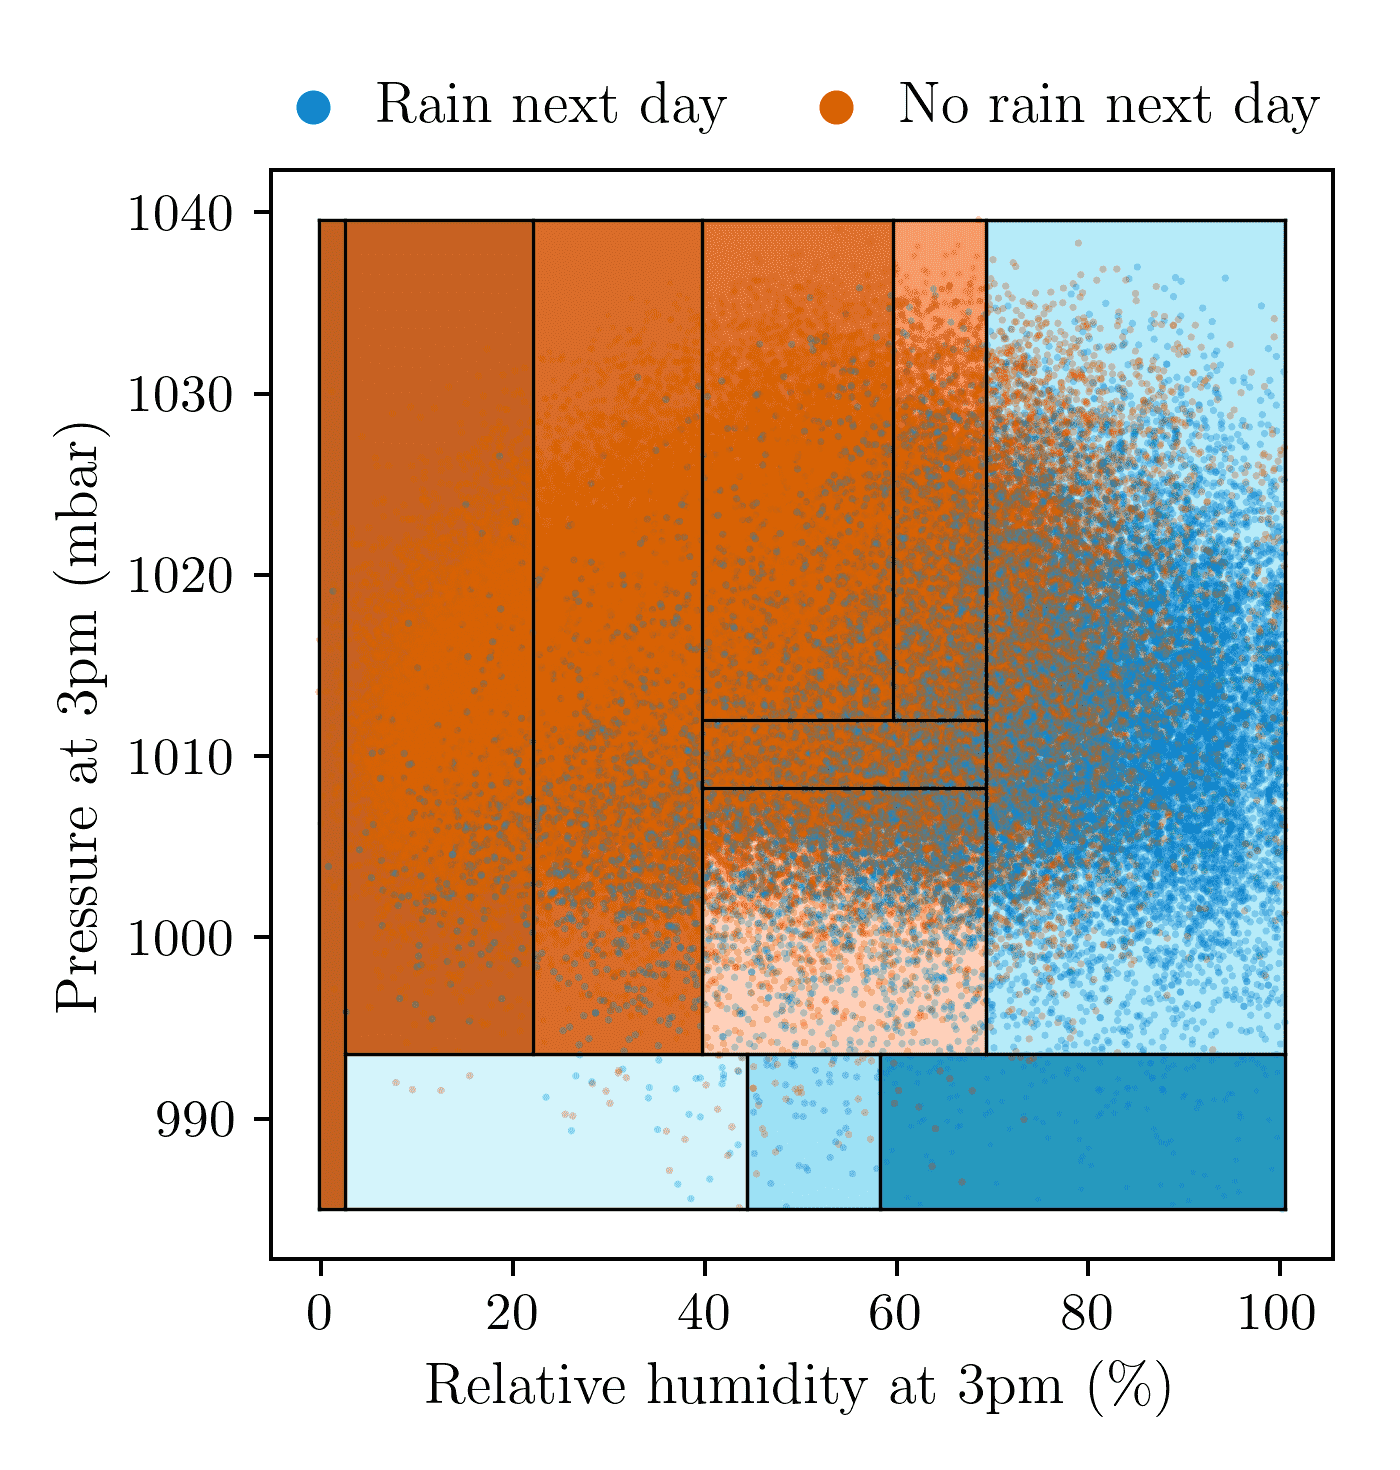
\includegraphics[scale=0.64]{graphics/weather_data_filled_partition.png}%
  \end{subfigure}
  \caption[Australian weather forecasting data]{
    Australian weather forecasting data. Left: colors indicate the response
    variable of dry (orange) or wet (blue) on the following
    day. Right: the data is overlaid with a Mondrian random tree,
    fitted with a lifetime of $\lambda = 5$
    selected by generalized cross-validation. Cell colors represent the response
  proportions.}
  \label{fig:mondrian_weather_data}
\end{figure}

We consider the classification problem of predicting whether or not it will
rain on the following day using two covariates: the percentage relative
humidity, and the pressure in mbar, both at 3pm on the current day. For the
purpose of framing this as a nonparametric regression problem, we consider
estimating the probability of rain as the regression function by setting
$Y_i = 1$ if there is rain on the following day and $Y_i = 0$ otherwise.
Outliers with pressure less than 985\,mbar or more than 1040\,mbar are removed
to justify the assertion in Assumption~\ref{ass:mondrian_data} that the density
of the covariates should be bounded away from zero, and the features are
linearly scaled to provide normalized samples
$(X_i, Y_i) \in [0, 1]^2 \times \{0, 1\}$.
We fit a Mondrian random forest to the data as defined in
Section~\ref{sec:mondrian_forests}, selecting the lifetime parameter with the
generalized cross-validation (GCV) method detailed in
Section~\ref{sec:mondrian_lifetime_selection}.

Figure~\ref{fig:mondrian_weather_data} plots the
data, using colors to indicate the response values, and illustrates how a
single Mondrian tree is fitted by sampling from an independent Mondrian process
and then computing local averages (equivalent to response proportions in this
special setting with binary outcomes) within each cell. The general pattern of
rain being predicted by high humidity and low pressure is apparent, with the
preliminary tree estimator taking the form of a step function on axis-aligned
rectangles. This illustrates the first-order bias of Mondrian random trees
discussed in Section~\ref{sec:mondrian_clt}, with the piecewise constant
estimator providing a poor approximation for the smooth true regression
function.

\begin{figure}[t]
  \centering
  \begin{subfigure}{0.49\textwidth}
    \centering
    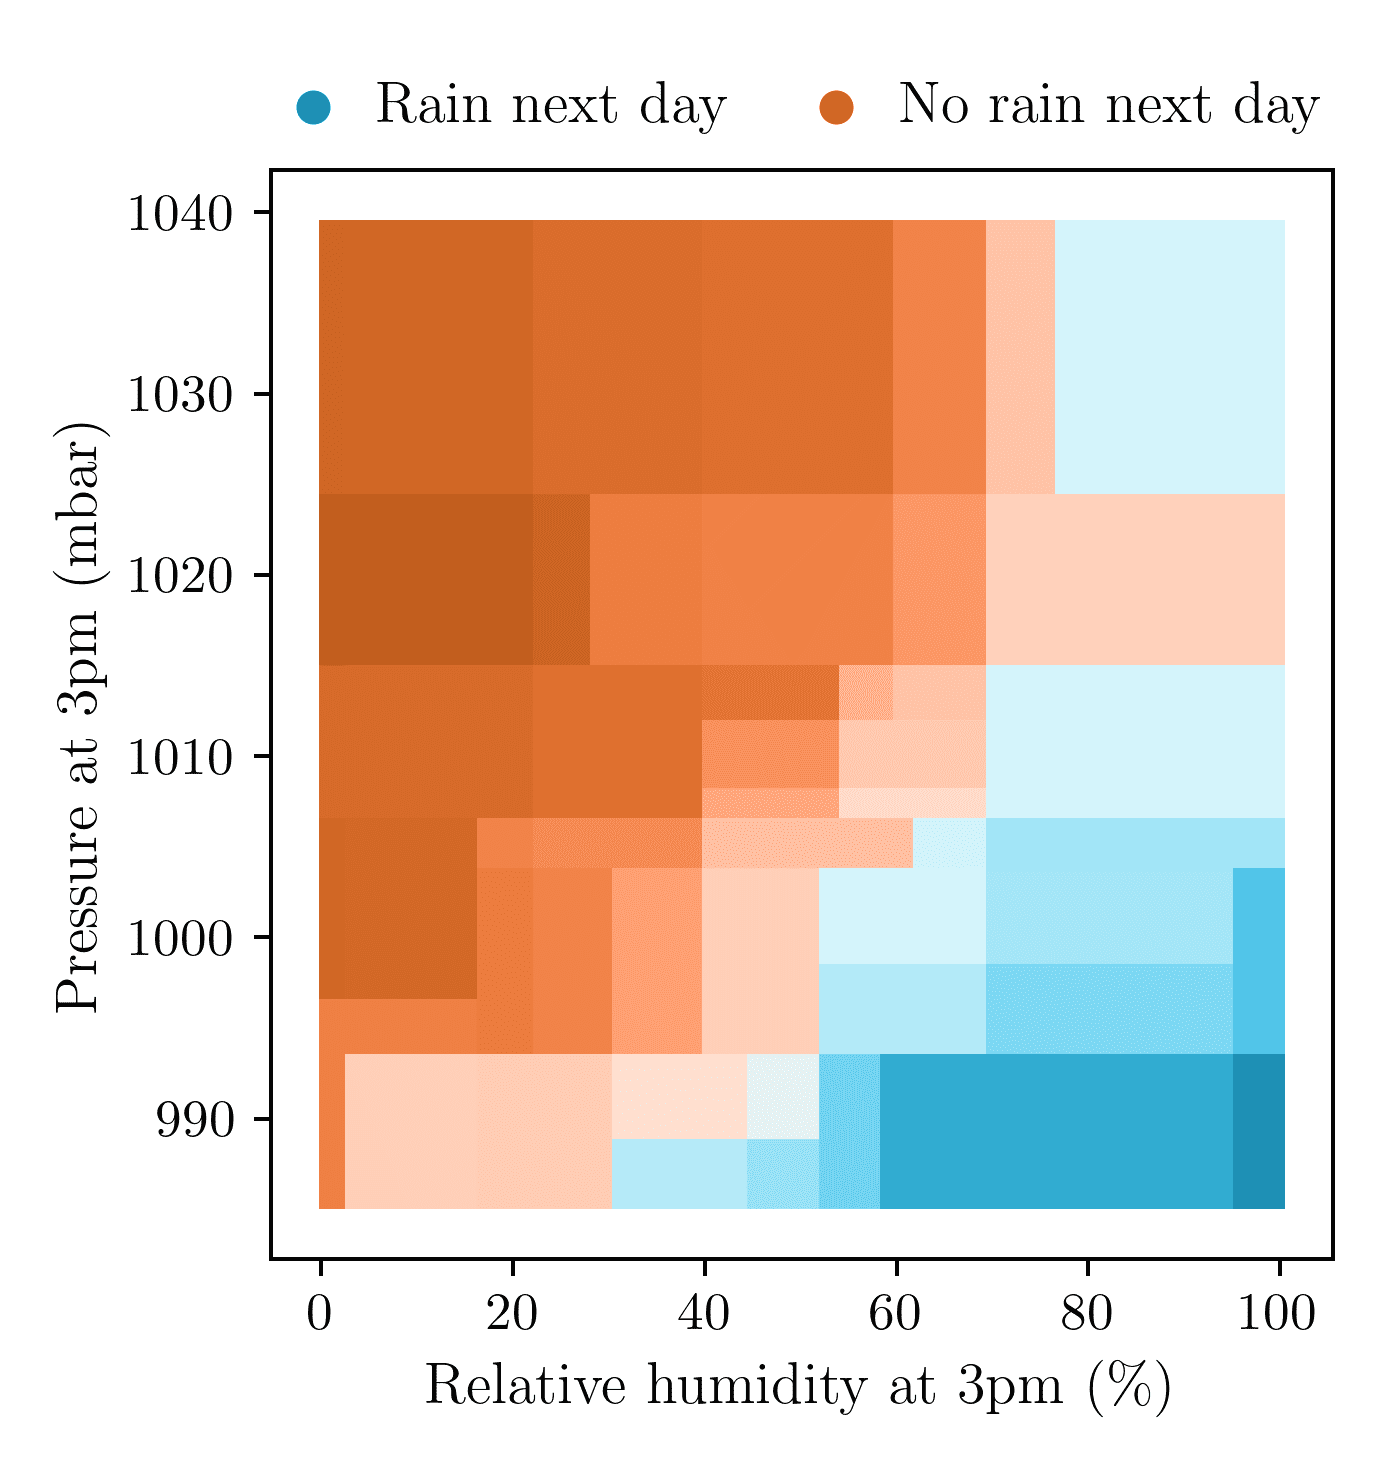
\includegraphics[scale=0.64]{graphics/weather_forest_2.png}%
  \end{subfigure}
  \begin{subfigure}{0.49\textwidth}
    \centering
    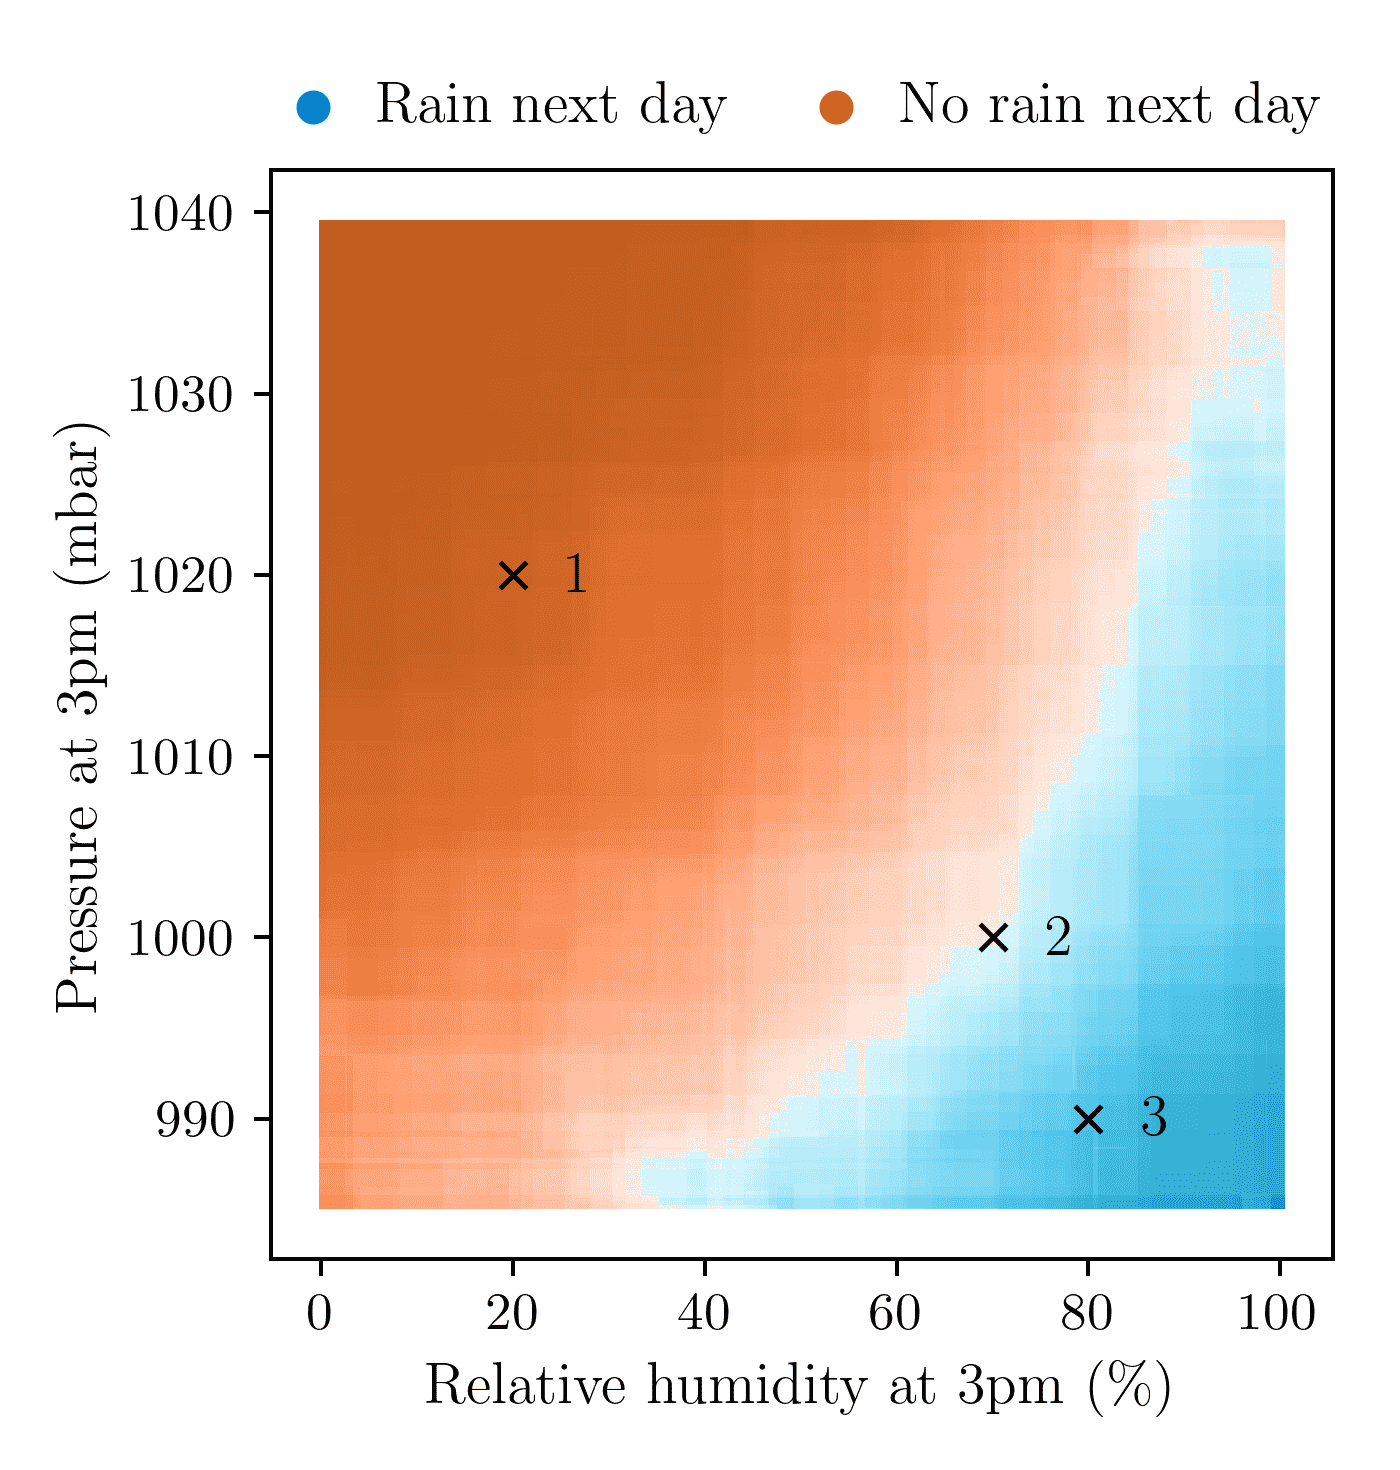
\includegraphics[scale=0.64]{graphics/weather_forest_design.png}%
  \end{subfigure}
  \caption[Fitting Mondrian random forests to the Australian weather data]{
    Fitting Mondrian random forests to the Australian weather data.
    Left: with $B=2$ trees, individual cells are clearly visible and the step
    function persists. Right: with $B=40$ trees, the estimate is much smoother
    as the individual tree estimates average out.
  Three design points are identified for further analysis.}
  \label{fig:mondrian_weather_forest}
\end{figure}

Figure~\ref{fig:mondrian_weather_forest} adds more trees to the estimator,
demonstrating the effect of increasing the forest size first to $B=2$
and then to $B=40$.
As more trees are included in the Mondrian random forest,
the regression estimate $\hat \mu(x)$ becomes smoother and therefore also
enjoys improved bias properties as shown in
Theorem~\ref{thm:mondrian_bias}, assuming a correct model specification.
We also choose three specific design points in the
(humidity, pressure) covariate space,
namely (20\%, 1020\,mbar), (70\%, 1000\,mbar), and (80\%, 990\,mbar),
at which to conduct inference
by constructing confidence intervals. See Table~\ref{tab:mondrian_weather_ci}
for the results.

\begin{figure}[t]
  \centering
  \begin{subfigure}{0.49\textwidth}
    \centering
    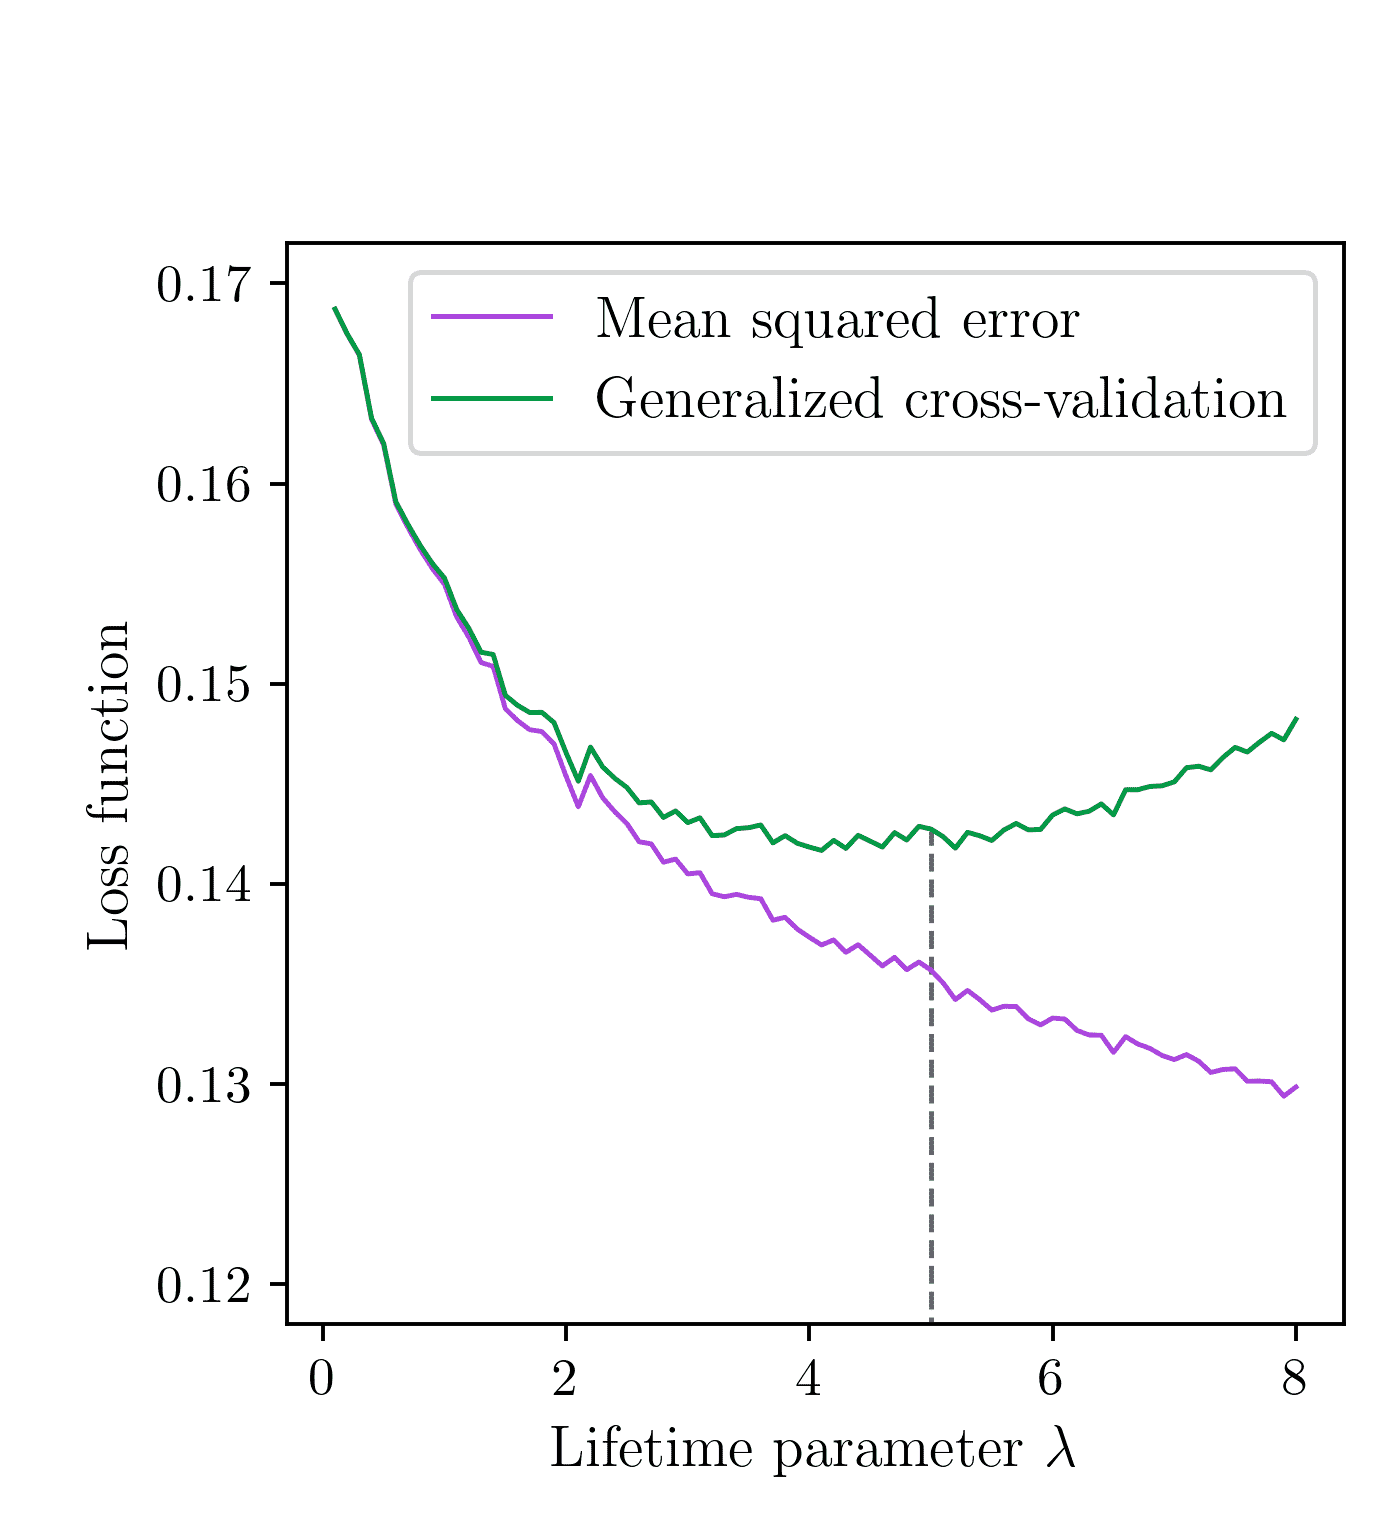
\includegraphics[scale=0.64]{graphics/weather_gcv.png}%
  \end{subfigure}
  \begin{subfigure}{0.49\textwidth}
    \centering
    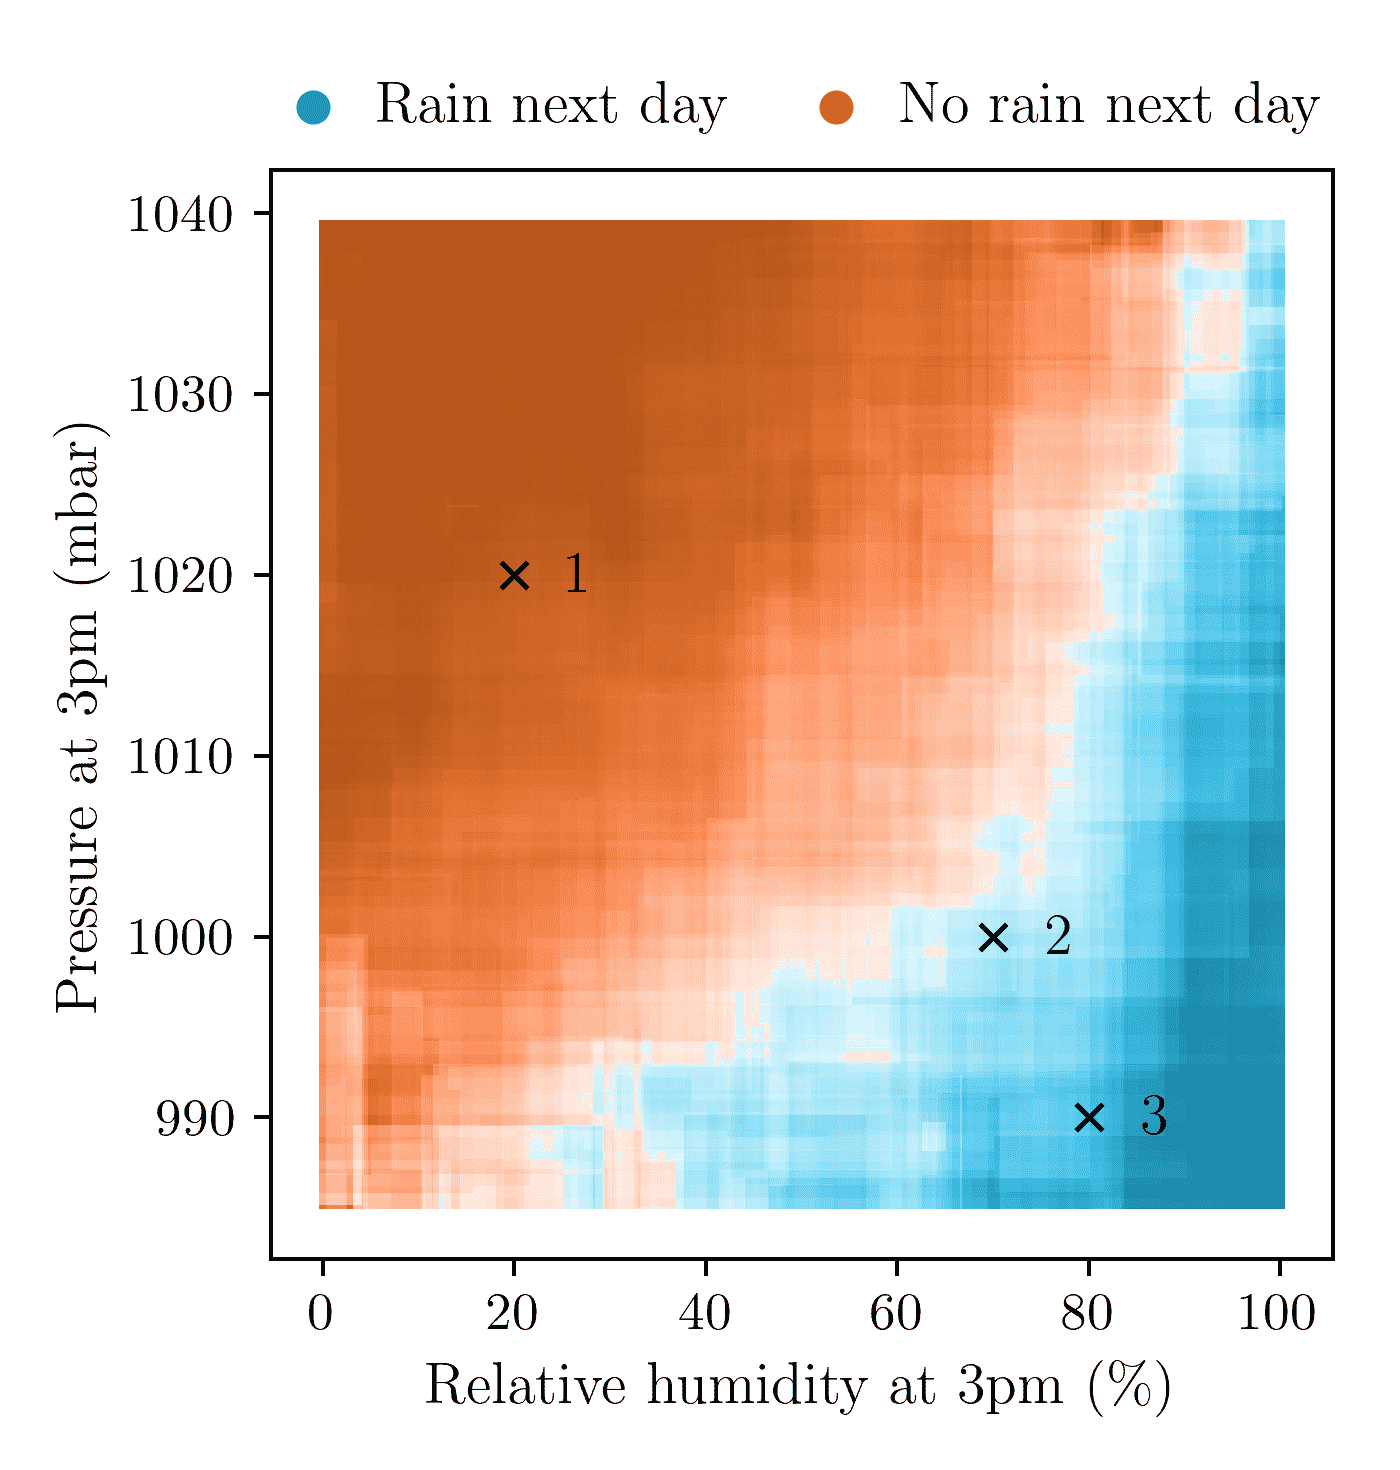
\includegraphics[scale=0.64]{graphics/weather_debiased_forest_design.png}%
  \end{subfigure}
  \caption[Cross-validation and debiasing for the Australian weather data]{
    Left: mean squared error and generalized cross-validation scores
    for Mondrian random forests with the Australian weather data.
    Right: a debiased Mondrian random forest with $B=20$, giving $40$ trees
  in total. Three design points are identified for further analysis.}
  \label{fig:mondrian_weather_gcv}
\end{figure}

In Figure~\ref{fig:mondrian_weather_gcv} we show the mean squared error and GCV scores
computed using \eqref{eq:mondrian_gcv} with $B=400$ trees
for several candidate lifetime parameters $\lambda$. As
expected, the mean squared error decreases monotonically
as $\lambda$ increases and the model
overfits, but the GCV score is minimized at a value which appropriately
balances the bias and variance; we take $\lambda = 5$.
We then fit a debiased Mondrian forest
with bias correction order $J = 1$ as described in
Section~\ref{sec:mondrian_debiased}, using $B=20$ trees at each debiasing level
$r \in \{0, 1\}$ for a total of $40$ trees.
We continue to use the same lifetime parameter
$\lambda = 5$ selected through GCV without debiasing, following the approach
recommended in Section~\ref{sec:mondrian_lifetime_selection} to ensure valid inference
through negligible bias.
The resulting debiased Mondrian random forest estimate is noticeably
less smooth than the version without bias correction.
This is expected due to both the inflated variance resulting from the debiasing
procedure, and the undersmoothing enacted by selecting a lifetime parameter
using GCV on the original estimator without debiasing.

\begin{table}[b!]
  \centering
  \begin{tabular}{|c|c|c|c|c|c|c|}
    \hline
    \multirow{2}{*}{Point}
    & \multirow{2}{*}{Humidity}
    & \multirow{2}{*}{Pressure}
    & \multicolumn{2}{|c|}{No debiasing, $J=0$}
    & \multicolumn{2}{|c|}{Debiasing, $J=1$} \\
    \cline{4-7}
    & &
    & $\hat\mu(x)$ & 95\% CI
    & $\hat\mu(x)$ & 95\% CI \\
    \hline
    $1$ & $20\%$ & $1020\,\textrm{mbar}$ &
    $\phantom{0}4.2\%$ &
    $3.9\%$ -- $4.5\%$ &
    $\phantom{0}2.0\%$ &
    $1.6\%$ -- $2.4\%$ \\
    $2$ & $70\%$ & $1000\,\textrm{mbar}$ &
    $52.6\%$ &
    $51.7\%$ -- $53.6\%$ &
    $59.8\%$ &
    $57.8\%$ -- $61.9\%$ \\
    $3$ & $80\%$ & $\phantom{1}990\,\textrm{mbar}$ &
    $78.1\%$ &
    $75.0\%$ -- $81.2\%$ &
    $93.2\%$ &
    $86.7\%$ -- $99.6\%$ \\
    \hline
  \end{tabular}
  \caption[Results for the Australian weather data]{
    Results for the Australian weather data
  at three specified design points.}
  \label{tab:mondrian_weather_ci}
\end{table}

Table~\ref{tab:mondrian_weather_ci} presents numerical results for estimation and
inference at the three specified design points. We first give the outcomes
without debiasing, using a Mondrian random forest with $B = 400$ trees and
$\lambda = 5$ selected by GCV. We then show the results with a first-order
($J=1$) debiased Mondrian random forest using $B = 200$ (again a total of
$400$ trees) and the same value of $\lambda = 5$. The predicted chance of rain
$\hat\mu(x)$ is found to vary substantially across different covariate values,
and the resulting confidence intervals (CI) are generally narrow due to the
large sample size and moderate lifetime parameter. The forest with debiasing
exhibits more extreme predictions away from $50\%$ and wider confidence
intervals in general, in line with the illustration in
Figure~\ref{fig:mondrian_weather_gcv}. Interestingly, the confidence intervals for the
non-debiased and debiased estimators do not intersect, indicating that the
original estimator is severely biased, and providing further justification for
our modified debiased random forest estimator.

\section{Conclusion}%
\label{sec:mondrian_conclusion}

We presented a central limit theorem for the Mondrian random forest estimator
and showed how to perform statistical inference on an unknown nonparametric
regression function. We introduced debiased versions of the Mondrian random
forest, exploiting any available higher-order smoothness, and demonstrated
their advantages
for statistical inference and their minimax optimality properties. We discussed
tuning parameter selection, enabling fully feasible and practical estimation
and inference procedures. An application to weather forecasting
in Australia was presented
as an illustrative example. Implementations of this chapter's methodology,
along with replication files for the empirical results, are provided by a Julia
package available at \github{wgunderwood/MondrianForests.jl}.
This work is based on \citet{cattaneo2023inference}, and has been
presented by Underwood at the University of Illinois Statistics Seminar (2024),
the University of Michigan Statistics Seminar (2024), and the University of
Pittsburgh Statistics Seminar (2024).
